%! Author = crist
%! Date = 26/10/2026

\spacing{1.3}
%----------------------------------------------------------------------------------------
%	UNIDAD 13: LUZ Y SONIDO, ONDAS QUE TRANSFIEREN ENERGÍA (4.º ESO)
%   Figuras: images/UD13/*.pdf (fuente HTML en images/UD13/html, SVG en images/UD13/svg)
%   Gráficas con pgfplots: estilo «grafica», definido al inicio de la UD1/UD7.
%   Datos usados en toda la unidad: v(sonido en el aire) = 340 m/s (salvo que se indique otro valor);
%   v(sonido en el agua de mar) = 1531 m/s; c = 3·10^8 m/s; n(agua) = 1,33.
%----------------------------------------------------------------------------------------
\providecommand{\sen}{\operatorname{sen}}

% Mapa conceptual del tema (fuente en images/mapas_conceptuales/html/temas.js)
\begin{figure}[H]
    \centering
    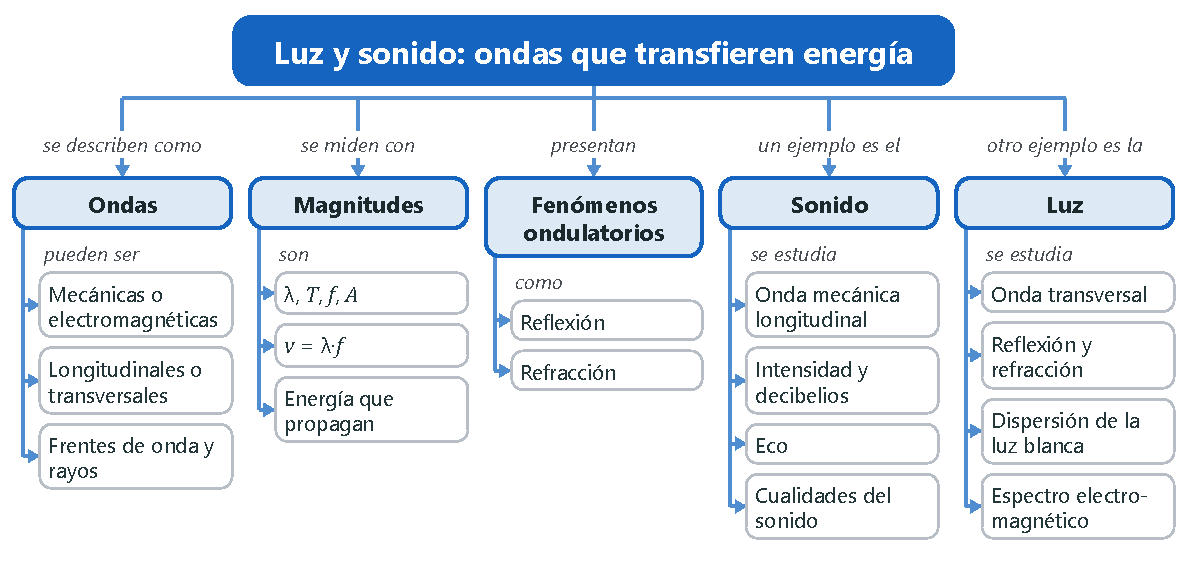
\includegraphics[width=\textwidth]{images/mapas_conceptuales/mapa_UD13}
\end{figure}

%========================================================================================
%\section*{Para empezar: la contaminación acústica}
%\addcontentsline{toc}{section}{Para empezar: la contaminación acústica}
%========================================================================================
%
%El \textbf{ruido} es cualquier sonido que no deseamos oír y que nos resulta molesto. Cuando es intenso y continuo, deteriora la calidad de vida: hablamos entonces de \textbf{contaminación acústica}. La Organización Mundial de la Salud (OMS) recomienda que el nivel de ruido ambiental en las calles no supere los \qty{65}{\decibel}, y España está entre los países más ruidosos de Europa, sobre todo por el tráfico.
%
%El ruido es un contaminante peculiar:
%\begin{itemize}
%    \item Producirlo es barato y no deja residuos: no contamina el aire, el agua ni el suelo.
%    \item Su radio de acción es pequeño comparado con el de otros contaminantes.
%    \item Solo lo percibimos por un sentido, el oído.
%\end{itemize}
%
%Sin embargo, sus efectos sobre la salud son importantes. Los \textbf{fisiológicos} pueden ser \emph{auditivos} (pérdida de audición, sordera) o \emph{no auditivos} (alteraciones del ritmo cardiaco, hipertensión, problemas de riego cerebral). Los \textbf{psicológicos} incluyen un sueño menos profundo, pérdida de memoria, estrés, irritabilidad, ansiedad o dolor de cabeza.
%
%Reducir la contaminación acústica contribuye a dos Objetivos de Desarrollo Sostenible: el \textbf{ODS 3} (\emph{Salud y bienestar}), en concreto la meta 3.4, que busca reducir la mortalidad por enfermedades no transmisibles, y el \textbf{ODS 11} (\emph{Ciudades y comunidades sostenibles}), cuya meta 11.6 pretende reducir el impacto ambiental negativo de las ciudades.
%
%En esta unidad estudiaremos qué son las \textbf{ondas}, cómo transportan energía sin transportar materia y cuáles son las propiedades de las dos ondas más presentes en nuestra vida: el \textbf{sonido} y la \textbf{luz}.
%
%\begin{exercise}
%    ¿Estás de acuerdo en que el ruido se considere un tipo de contaminación? Razona tu respuesta.
%    \begin{solu}
%        Respuesta libre. \textcolor{red}{Sí}: aunque no deja residuos, el ruido empeora la calidad de vida y tiene efectos negativos sobre la salud física y psicológica, igual que otros contaminantes.
%    \end{solu}
%\end{exercise}
%
%\begin{exercise}
%    ¿Qué ruidos contribuyen más a la contaminación acústica en tu entorno (en casa, en el instituto, en tu barrio)?
%    \begin{solu}
%        Respuesta libre. Por ejemplo: el \textcolor{red}{tráfico} de las calles cercanas, las voces y gritos en clase y en los pasillos, el volumen alto de los altavoces y auriculares, las obras, los bares o las motos.
%    \end{solu}
%\end{exercise}
%
%\begin{exercise}
%    ¿En qué se diferencia la contaminación acústica de otros tipos de contaminación, como la del aire o la del agua?
%    \begin{solu}
%        Su producción es \textcolor{red}{barata} y \textcolor{red}{no genera residuos}; su \textcolor{red}{radio de acción es pequeño}; no contamina el aire, el agua ni el suelo, y se percibe por un \textcolor{red}{único sentido}, el oído. Cuando cesa la fuente, desaparece la contaminación.
%    \end{solu}
%\end{exercise}
%
%\begin{exercise}
%    ¿Te parece adecuado que el nivel máximo recomendado de ruido ambiental sea de \qty{65}{\decibel}? ¿Debería ser mayor o menor?
%    \begin{solu}
%        Respuesta libre. Es un \textcolor{red}{límite razonable} para la calle; en lugares de descanso, de estudio o durante la noche debería ser \textcolor{red}{bastante menor} (la OMS recomienda unos \qty{35}{\decibel} en las aulas y aún menos en los dormitorios).
%    \end{solu}
%\end{exercise}
%
%\begin{exercise}
%    ¿Cuáles de los efectos del ruido sobre la salud te parecen más importantes? Clasifícalos en fisiológicos y psicológicos.
%    \begin{solu}
%        \textbf{Fisiológicos}: auditivos (pérdida de audición y sordera) y no auditivos (alteraciones del ritmo cardiaco, hipertensión arterial, afecciones en el riego cerebral). \textbf{Psicológicos}: sueño menos profundo, pérdida de memoria, estrés, irritabilidad, ansiedad, mal humor, dolor de cabeza. La importancia de cada uno es respuesta libre.
%    \end{solu}
%\end{exercise}
%
%\begin{exercise}
%    Propón tres medidas para reducir el ruido en las ciudades y relaciónalas con las metas 3.4 y 11.6 de los ODS.
%    \begin{solu}
%        Respuesta libre. Por ejemplo: \textcolor{red}{limitar el tráfico} y la velocidad en el centro, usar \textcolor{red}{asfalto} y materiales que absorban el sonido, poner \textcolor{red}{pantallas acústicas} en las vías rápidas, prohibir el claxon salvo emergencias, plantar árboles o concienciar sobre el volumen de la voz y de los aparatos. Todas mejoran la salud (meta 3.4) y reducen el impacto ambiental de las ciudades (meta 11.6).
%    \end{solu}
%\end{exercise}

%========================================================================================
\section{¿Qué es una onda? El movimiento ondulatorio}
%========================================================================================

Si tiramos una piedra a un estanque, en el punto donde cae el agua empieza a vibrar, y esa vibración se transmite a las partículas de agua vecinas: se forman círculos que se alejan del punto de impacto. Algo parecido ocurre al comprimir unas espiras de un muelle sujeto a una pared, al agitar el extremo de una cuerda, cuando vibra la membrana de un altavoz o cuando el Sol emite luz. En todos los casos, una \textbf{perturbación} producida en un punto, llamado \textbf{foco}, se \textbf{propaga} y llega a otros puntos, a los que transmite energía.

\begin{figure}[H]
    \centering
    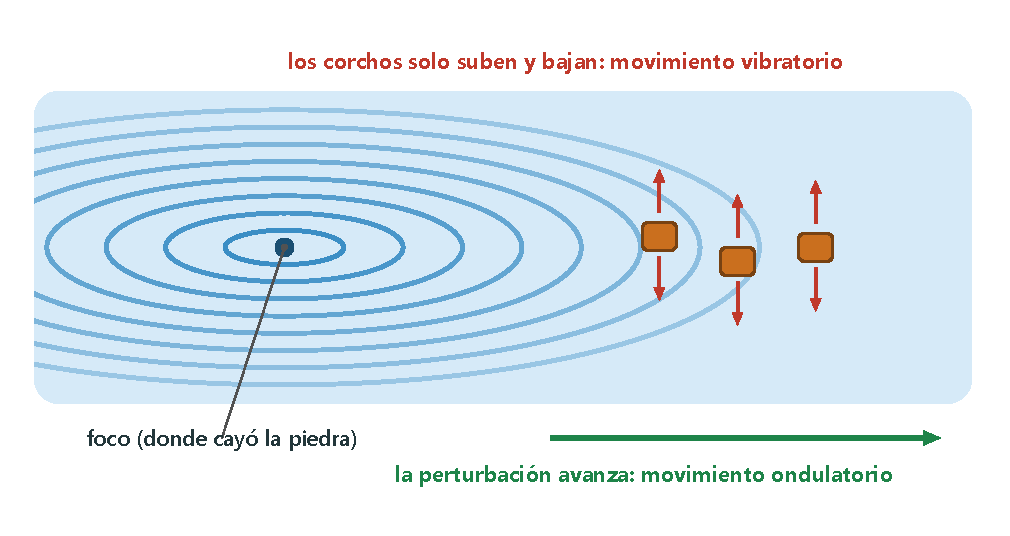
\includegraphics[width=0.75\textwidth]{images/UD13/corchos_agua}
    \caption{Unos corchos flotando en un estanque suben y bajan al llegar las ondas, pero no avanzan con ellas.}
    \label{fig:corchos_agua}
\end{figure}

Observa que los corchos de la figura~\ref{fig:corchos_agua} \emph{no se desplazan} hacia la orilla: solo suben y bajan alrededor de su posición. Lo que avanza no es el agua, sino la perturbación y, con ella, la energía.

\begin{definition}[Movimiento ondulatorio y onda]
    El \textbf{movimiento ondulatorio} es la propagación de un movimiento vibratorio (una perturbación) de unos puntos a otros de un medio. Es una forma de \textbf{transmitir energía sin transportar materia}.

    Una \textbf{onda} es la forma que adopta en cada instante la perturbación que se propaga.
\end{definition}

\begin{exercise}
    En la figura~\ref{fig:corchos_agua}, ¿qué movimiento es el vibratorio y cuál es el ondulatorio?
    \begin{solu}
        El \textcolor{red}{movimiento vibratorio} es el de cada corcho (y cada partícula de agua), que sube y baja alrededor de su posición de equilibrio. El \textcolor{red}{movimiento ondulatorio} es la propagación de esa vibración por la superficie del agua, alejándose del foco.
    \end{solu}
\end{exercise}

\begin{exercise}
    Si la onda no transporta materia, ¿cómo podemos saber que transporta energía? Pon un ejemplo.
    \begin{solu}
        Porque al llegar a un cuerpo \textcolor{red}{lo pone en movimiento} o lo modifica: las olas mueven una barca, el sonido hace vibrar el tímpano o los cristales de una ventana, y la luz del Sol calienta la piel.
    \end{solu}
\end{exercise}

\subsection{¿Cómo se clasifican las ondas?}

\textbf{Según necesiten o no un medio material para propagarse}:
\begin{itemize}
    \item \textbf{Ondas mecánicas}: se originan al perturbar un \emph{medio elástico} (sólido, líquido o gas) y \textbf{no pueden propagarse en el vacío}. Son mecánicas las ondas en la superficie del agua, el sonido y las ondas en cuerdas y muelles.
    \item \textbf{Ondas electromagnéticas}: \textbf{pueden propagarse en el vacío}, aunque también lo hacen por muchos medios materiales. Son ondas electromagnéticas la luz visible, los rayos X, los rayos ultravioleta e infrarrojos, las microondas y las ondas de radio.
\end{itemize}

\textbf{Según la relación entre la dirección de vibración y la de propagación}:
\begin{itemize}
    \item \textbf{Ondas transversales}: las partículas vibran \textbf{perpendicularmente} a la dirección en que avanza la onda. Forman una sucesión de \textbf{crestas} y \textbf{valles}. Son transversales las ondas en una cuerda, en la superficie del agua y las ondas electromagnéticas.
    \item \textbf{Ondas longitudinales}: las partículas vibran \textbf{en la misma dirección} en que avanza la onda. Forman una sucesión de \textbf{compresiones} y \textbf{dilataciones}. Son longitudinales el sonido y las compresiones que se propagan por un muelle.
\end{itemize}

\begin{figure}[H]
    \centering
    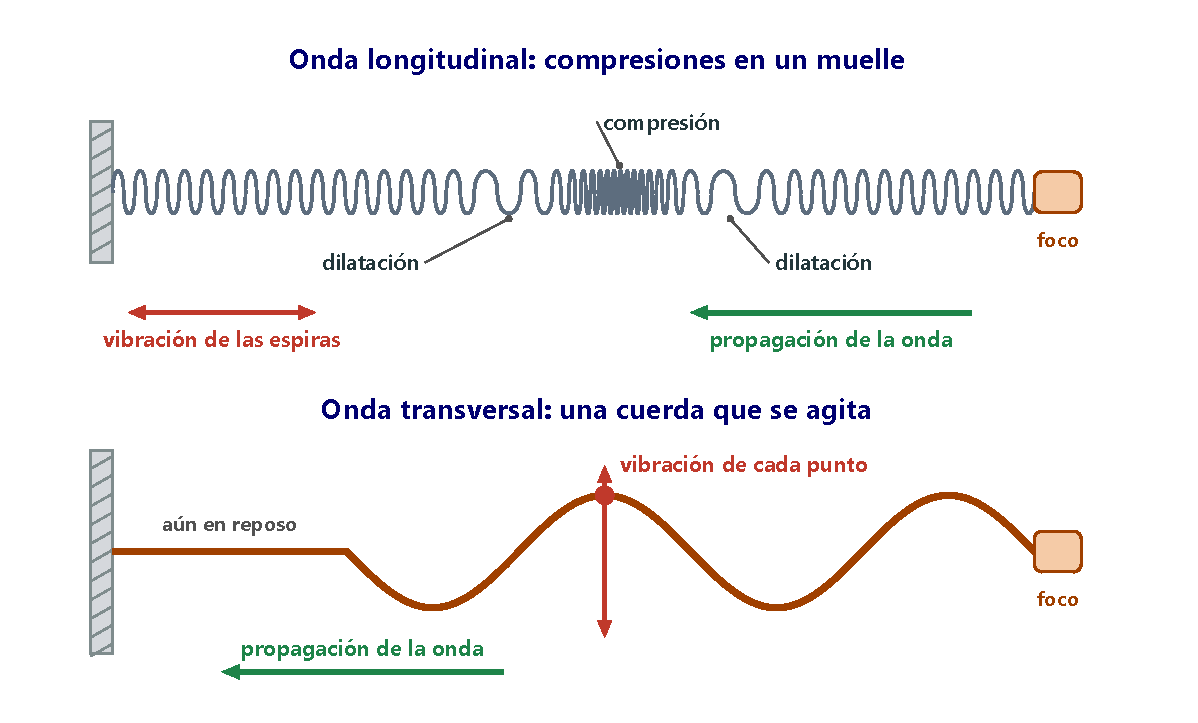
\includegraphics[width=0.9\textwidth]{images/UD13/tipos_ondas}
    \caption{Arriba, una onda longitudinal: las espiras vibran en la misma dirección en que avanza la compresión. Abajo, una onda transversal: cada punto de la cuerda sube y baja mientras la onda avanza en horizontal.}
    \label{fig:tipos_ondas}
\end{figure}

\begin{exercise}
    Indica si son verdaderas o falsas estas afirmaciones y justifícalo:
    \begin{enumerate}[label=\alph*)]
        \item Las ondas mecánicas necesitan un medio material para propagarse.
        \item Las ondas electromagnéticas no pueden propagarse por medios materiales.
        \item El sonido puede viajar por el vacío.
    \end{enumerate}
    \begin{solu}
        a) \textcolor{red}{Verdadera}: se propagan porque las partículas del medio se transmiten la vibración unas a otras. b) \textcolor{red}{Falsa}: pueden propagarse en el vacío, pero también por muchos medios materiales (la luz atraviesa el aire, el agua o el vidrio). c) \textcolor{red}{Falsa}: el sonido es una onda mecánica y necesita un medio material.
    \end{solu}
\end{exercise}

\subsection{¿Qué es un frente de onda? ¿Y un rayo?}

Cuando una onda se propaga en todas las direcciones desde un foco, todos los puntos que están a la misma distancia del foco son alcanzados a la vez por la perturbación.

\begin{definition}[Frente de onda y rayo]
    Un \textbf{frente de onda} es la línea o la superficie formada por todos los puntos alcanzados por la perturbación en el mismo instante.

    Un \textbf{rayo} es una línea imaginaria perpendicular a los frentes de onda que indica la dirección de propagación.
\end{definition}

Cerca de un foco puntual, los frentes de onda son esferas (o circunferencias en la superficie del agua); muy lejos del foco, un trozo de esa esfera es casi plano y se habla de \textbf{frentes de onda planos}, cuyos rayos son paralelos.

\begin{figure}[H]
    \centering
    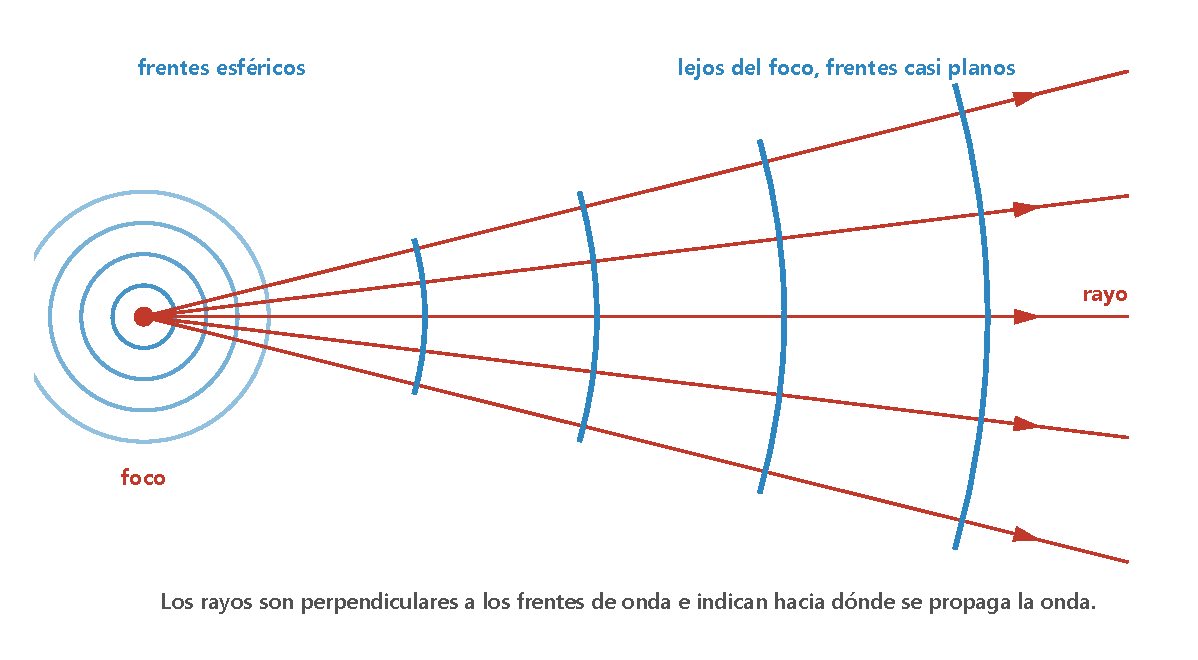
\includegraphics[width=0.85\textwidth]{images/UD13/frentes_rayos}
    \caption{Frentes de onda esféricos cerca del foco y casi planos lejos de él. Los rayos son perpendiculares a los frentes.}
    \label{fig:frentes_rayos}
\end{figure}

\begin{exercise}
    Un frente de onda plano avanza hacia la derecha. ¿Cómo son sus rayos? ¿Y si el frente avanza hacia abajo?
    \begin{solu}
        Los rayos son \textcolor{red}{rectas paralelas entre sí y perpendiculares al frente}, con el sentido de la propagación: si el frente avanza hacia la derecha (es un plano vertical), los rayos son \textcolor{red}{horizontales} y apuntan a la derecha; si avanza hacia abajo (el frente es horizontal), los rayos son \textcolor{red}{verticales} y apuntan hacia abajo.
    \end{solu}
\end{exercise}

\subsection{¿Cuáles son las magnitudes características de las ondas?}

\begin{figure}[H]
    \centering
    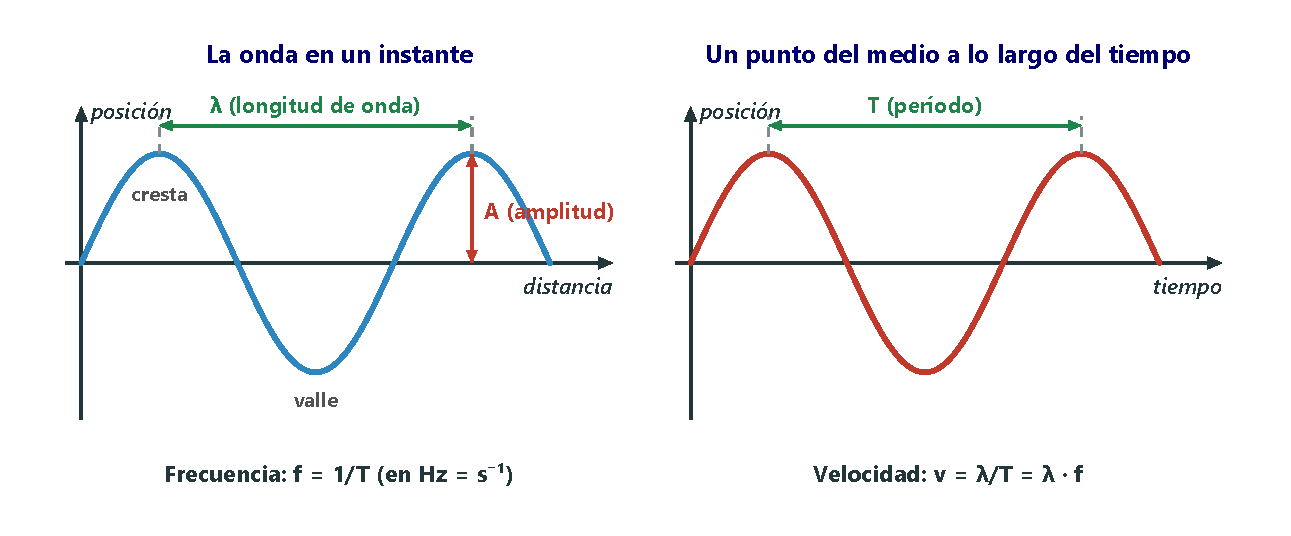
\includegraphics[width=\textwidth]{images/UD13/magnitudes_onda}
    \caption{Izquierda: la onda en un instante, con su amplitud y su longitud de onda. Derecha: la posición de un punto del medio a lo largo del tiempo, que se repite cada período.}
    \label{fig:magnitudes_onda}
\end{figure}

\begin{itemize}
    \item La \textbf{amplitud}, \(A\), es la separación máxima de cada punto del medio respecto de su posición de equilibrio. Se mide en metros.
    \item La \textbf{longitud de onda}, \(\lambda\), es la distancia entre dos puntos consecutivos que vibran exactamente igual (por ejemplo, dos crestas o dos valles seguidos). Es la distancia que avanza la onda mientras el foco realiza una vibración completa. Se mide en metros.
    \item El \textbf{período}, \(T\), es el tiempo que tarda un punto en hacer una vibración completa, que coincide con el que tarda la onda en avanzar una longitud de onda. Se mide en segundos.
    \item La \textbf{frecuencia}, \(f\), es el número de vibraciones que realiza cada punto en un segundo. Es la inversa del período, \(f = 1/T\), y se mide en \textbf{hercios} (\unit{\hertz}): \(\qty{1}{\hertz} = \qty{1}{\per\s}\).
\end{itemize}

\subsection{¿A qué velocidad se propagan las ondas?}

Si el medio tiene las mismas propiedades en todas las direcciones (es \textbf{isótropo}), la onda avanza con \textbf{velocidad constante}, es decir, con movimiento uniforme. La \textbf{velocidad de propagación}, \(v\), es la distancia que recorre la onda en cada unidad de tiempo:
\[ v = \frac{\text{distancia recorrida}}{\text{tiempo empleado}} \]

\begin{example}
    En el centro de una piscina circular de \qty{6}{\m} de radio se produce una perturbación en la superficie del agua, que tarda \qty{10}{\s} en llegar al borde. ¿A qué velocidad se propaga la onda?
    \[ v = \frac{\text{distancia}}{\text{tiempo}} = \frac{\qty{6}{\m}}{\qty{10}{\s}} = \textcolor{red}{\qty{0.6}{\m\per\s}} \]
\end{example}

\subsection{¿Cómo se relacionan las magnitudes de una onda?}

En un período, \(T\), la onda avanza exactamente una longitud de onda, \(\lambda\). Por tanto, su velocidad es \(v = \lambda / T\). Como la frecuencia es la inversa del período, obtenemos la \textbf{ecuación fundamental de las ondas}:
\begin{equation*}
    \boxed{v = \frac{\lambda}{T} = \lambda \cdot f}
\end{equation*}

\begin{remark}
    La velocidad de una onda depende del \textbf{medio} por el que se propaga, no del foco. La frecuencia, en cambio, la fija el \textbf{foco}. Por eso, cuando una onda pasa de un medio a otro, su frecuencia no cambia, pero sí su velocidad y su longitud de onda.
\end{remark}

\begin{example}
    Por una cuerda tensa se propaga, a \qty{25}{\m\per\s}, una onda de \qty{0.5}{\m} de longitud de onda. Calcula su frecuencia y su período.
    \[ f = \frac{v}{\lambda} = \frac{\qty{25}{\m\per\s}}{\qty{0.5}{\m}} = \textcolor{red}{\qty{50}{\hertz}}; \qquad T = \frac{1}{f} = \frac{1}{\qty{50}{\hertz}} = \textcolor{red}{\qty{0.02}{\s}} \]
\end{example}

\begin{exercise}
    Por una cuerda se propaga, a \qty{12}{\m\per\s}, un tren de ondas de \qty{1.5}{\m} de longitud de onda. ¿Cuáles son su frecuencia y su período?
    \begin{solu}
        \(f = \dfrac{v}{\lambda} = \dfrac{12}{\num{1.5}} = \textcolor{red}{\qty{8}{\hertz}}\); \(T = \dfrac{1}{f} = \dfrac{1}{8} = \textcolor{red}{\qty{0.125}{\s}}\).
    \end{solu}
\end{exercise}

\begin{exercise}
    Una emisora de radio de FM emite con una frecuencia de \qty{100}{\mega\hertz}. Si las ondas de radio viajan a \qty{3e8}{\m\per\s}, ¿cuál es su longitud de onda?
    \begin{solu}
        \(\lambda = \dfrac{v}{f} = \dfrac{\num{3e8}}{\num{1e8}} = \textcolor{red}{\qty{3}{\m}}\).
    \end{solu}
\end{exercise}

\subsection{Las ondas propagan energía}

En un movimiento ondulatorio se propaga energía, pero no materia. Para medir la rapidez con la que la onda transporta energía a través de una superficie se define la intensidad.

\begin{definition}[Intensidad de una onda]
    La \textbf{intensidad}, \(I\), de una onda es la energía que atraviesa cada unidad de superficie, colocada perpendicularmente a la dirección de propagación, en cada unidad de tiempo. Equivale a la potencia por unidad de superficie y se mide en \unit{\watt\per\square\m}:
    \[ I = \frac{E}{t \cdot S} = \frac{P}{S} \]
\end{definition}

Si un foco emite por igual en todas las direcciones, a una distancia \(r\) la energía se reparte sobre una esfera de superficie \(S = 4\pi r^2\). Por tanto:
\begin{equation*}
    \boxed{I = \frac{P}{4\pi r^2}}
\end{equation*}
La intensidad es \textbf{inversamente proporcional al cuadrado de la distancia} al foco: al doble de distancia, la intensidad es la cuarta parte; al triple, la novena parte.

\begin{figure}[H]
    \centering
    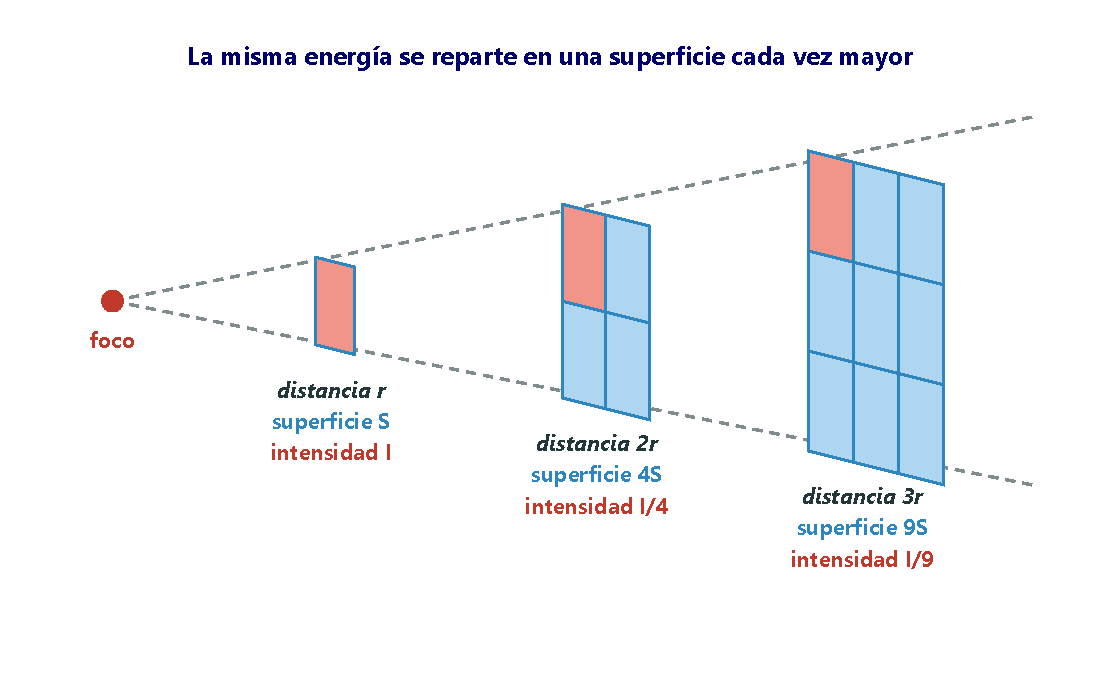
\includegraphics[width=0.75\textwidth]{images/UD13/intensidad_distancia}
    \caption{Al alejarse del foco, la misma energía se reparte en una superficie mayor y la intensidad disminuye.}
    \label{fig:intensidad_distancia}
\end{figure}

\begin{example}
    Un altavoz emite una potencia sonora de \qty{2}{\watt} por igual en todas las direcciones. ¿Con qué intensidad llega el sonido a \qty{5}{\m}? ¿Y a \qty{10}{\m}?
    \[ I_1 = \frac{P}{4\pi r^2} = \frac{\qty{2}{\watt}}{4\pi \cdot (\qty{5}{\m})^2} = \textcolor{red}{\qty{6.4e-3}{\watt\per\square\m}} \]
    Al doble de distancia, la intensidad es la cuarta parte: \(I_2 = I_1/4 = \textcolor{red}{\qty{1.6e-3}{\watt\per\square\m}}\).
\end{example}

\subsection{Fenómenos ondulatorios: reflexión y refracción}

Para explicar qué ocurre cuando una onda llega a un obstáculo o a otro medio, usamos los rayos y la \textbf{normal}, una recta perpendicular a la superficie en el punto donde llega el rayo. El \textbf{ángulo de incidencia}, \(i\), es el que forma el rayo incidente con la normal.

\begin{definition}[Reflexión]
    La \textbf{reflexión} es el cambio de dirección que experimenta una onda al chocar con una superficie sin atravesarla. La onda reflejada sigue en el mismo medio y, por tanto, con la misma velocidad.
\end{definition}

\begin{marker}
    \textbf{Leyes de la reflexión}
    \begin{itemize}
        \item El rayo incidente, la normal y el rayo reflejado están en el mismo plano.
        \item El ángulo de incidencia es igual al ángulo de reflexión (el que forma el rayo reflejado con la normal): \(\hat{\imath} = \hat{r}\).
    \end{itemize}
\end{marker}

\begin{definition}[Refracción]
    La \textbf{refracción} es el cambio de velocidad, y en general de dirección, que experimenta una onda al pasar de un medio a otro en el que se propaga con distinta velocidad.
\end{definition}

\begin{figure}[H]
    \centering
    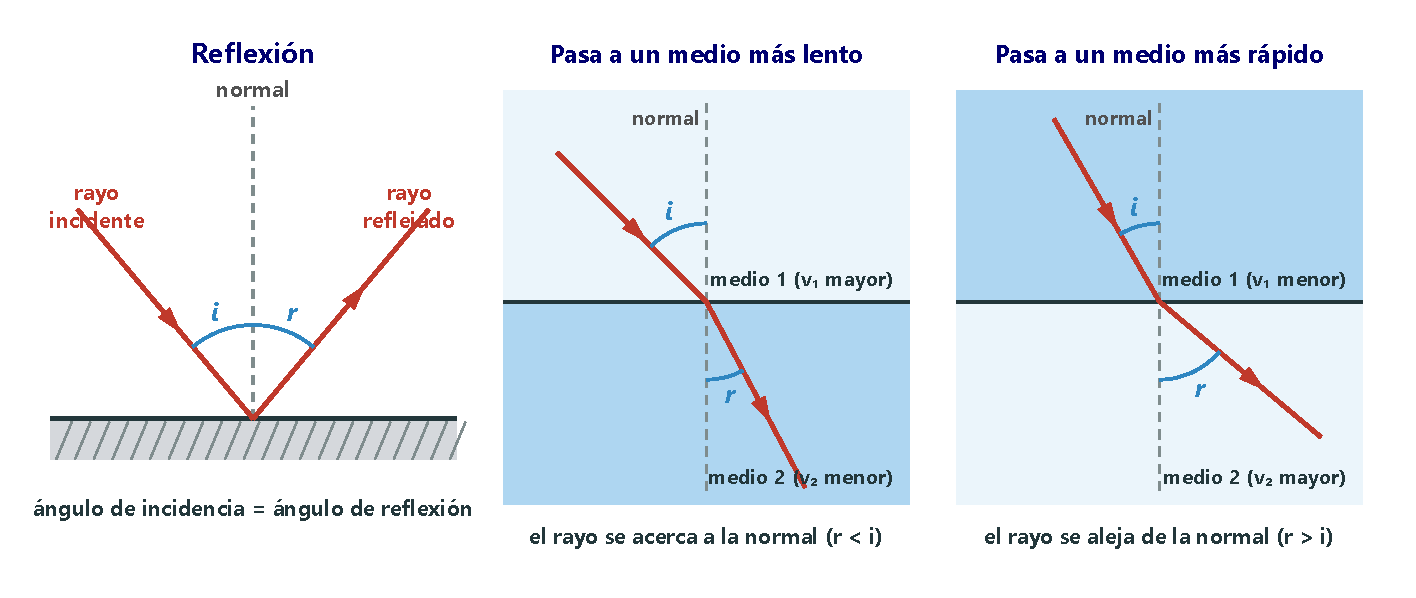
\includegraphics[width=\textwidth]{images/UD13/reflexion_refraccion}
    \caption{Reflexión (izquierda) y refracción de una onda al pasar a un medio en el que es más lenta (centro) o más rápida (derecha).}
    \label{fig:reflexion_refraccion}
\end{figure}

\begin{marker}
    \textbf{Leyes de la refracción}
    \begin{itemize}
        \item El rayo incidente, la normal y el rayo refractado están en el mismo plano.
        \item Si la onda pasa a un medio en el que se propaga \textbf{más despacio}, el rayo refractado \textbf{se acerca a la normal}. Si pasa a un medio en el que va \textbf{más deprisa}, \textbf{se aleja de la normal}.
        \item Si la onda llega \textbf{perpendicularmente} a la superficie de separación, no se desvía: sigue en línea recta (aunque cambia su velocidad).
    \end{itemize}
\end{marker}

\begin{exercise}
    Un rayo llega a una superficie formando \ang{35} con la normal. ¿Qué ángulo forma el rayo reflejado con la normal? ¿Y con la superficie?
    \begin{solu}
        Con la normal, \textcolor{red}{\ang{35}} (ley de la reflexión). Con la superficie, \(\ang{90} - \ang{35} = \textcolor{red}{\ang{55}}\).
    \end{solu}
\end{exercise}

%----------------------------------------------------------------------------------------
\subsection*{Actividades de consolidación: el movimiento ondulatorio}
%----------------------------------------------------------------------------------------

\begin{exercise}
    Clasifica estas ondas según necesiten o no un medio material y según sean transversales o longitudinales:
    \begin{enumerate}[label=\alph*)]
        \item Las ondas en la superficie de un lago.
        \item El sonido.
        \item Las ondas en una cuerda de guitarra.
        \item La luz.
        \item Las compresiones que recorren un muelle.
    \end{enumerate}
    \begin{solu}
        a) \textcolor{red}{Mecánica y transversal}. b) \textcolor{red}{Mecánica y longitudinal}. c) \textcolor{red}{Mecánica y transversal}. d) \textcolor{red}{Electromagnética y transversal}. e) \textcolor{red}{Mecánica y longitudinal}.
    \end{solu}
\end{exercise}

\begin{exercise}
    Sujetamos un extremo de un muelle a la pared y comprimimos unas espiras del otro extremo. Describe en cuatro pasos lo que ocurre a continuación.
    \begin{solu}
        1) Las espiras comprimidas empujan a las siguientes. 2) La \textcolor{red}{compresión avanza} por el muelle hacia la pared, mientras las espiras que ya ha pasado vuelven a su posición. 3) Cada espira solo \textcolor{red}{vibra adelante y atrás}, en la misma dirección en que avanza la compresión. 4) La compresión llega a la pared: se ha propagado la perturbación (y la energía), pero \textcolor{red}{no la materia} del muelle. Es una onda longitudinal.
    \end{solu}
\end{exercise}

\begin{exercise}
    Relaciona cada concepto con su definición:
    \begin{center}
        % --- tabla antigua ---
        % \begin{tblr}{colspec={lX}, width=\linewidth, hlines, vlines, row{1}={bg=ocre!85, fg=white, font=\bfseries}, cells={font=\small}}
            % Concepto & Definición \\
            % a) Movimiento ondulatorio & 1. Onda en la que las partículas vibran en la dirección de propagación. \\
            % b) Onda & 2. Propagación de un movimiento vibratorio. \\
            % c) Onda longitudinal & 3. Onda que necesita un medio material. \\
            % d) Frente de onda & 4. Onda en la que las partículas vibran perpendicularmente a la dirección de propagación. \\
            % e) Longitud de onda & 5. Superficie formada por los puntos alcanzados por la perturbación en el mismo instante. \\
            % f) Rayo & 6. Línea perpendicular al frente de onda. \\
            % g) Onda mecánica & 7. Separación máxima de un punto respecto de su posición de equilibrio. \\
            % h) Período & 8. Distancia entre dos puntos consecutivos que vibran de la misma manera. \\
            % i) Onda transversal & 9. Forma que adopta en cada instante la perturbación. \\
            % j) Amplitud & 10. Tiempo que tarda la perturbación en recorrer una longitud de onda. \\
        % \end{tblr}
        % --- tabla nueva ---
        {\small
        \begin{tabular}{@{}l p{0.78\linewidth}@{}}
            \toprule
            \textbf{Concepto} & \textbf{Definición} \\
            \midrule
            a) Movimiento ondulatorio & 1. Onda en la que las partículas vibran en la dirección de propagación. \\[3pt]
            b) Onda & 2. Propagación de un movimiento vibratorio. \\[3pt]
            c) Onda longitudinal & 3. Onda que necesita un medio material. \\[3pt]
            d) Frente de onda & 4. Onda en la que las partículas vibran perpendicularmente a la dirección de propagación. \\[3pt]
            e) Longitud de onda & 5. Superficie formada por los puntos alcanzados por la perturbación en el mismo instante. \\[3pt]
            f) Rayo & 6. Línea perpendicular al frente de onda. \\[3pt]
            g) Onda mecánica & 7. Separación máxima de un punto respecto de su posición de equilibrio. \\[3pt]
            h) Período & 8. Distancia entre dos puntos consecutivos que vibran de la misma manera. \\[3pt]
            i) Onda transversal & 9. Forma que adopta en cada instante la perturbación. \\[3pt]
            j) Amplitud & 10. Tiempo que tarda la perturbación en recorrer una longitud de onda. \\
            \bottomrule
        \end{tabular}
        }
    \end{center}
    \begin{solu}
        \textcolor{red}{a-2, b-9, c-1, d-5, e-8, f-6, g-3, h-10, i-4, j-7}.
    \end{solu}
\end{exercise}

\begin{exercise}
    Un punto de un medio vibra con un período de \qty{0.04}{\s}.
    \begin{enumerate}[label=\alph*)]
        \item ¿Cuál es su frecuencia?
        \item ¿Cuántas vibraciones completa en un minuto y medio?
    \end{enumerate}
    \begin{solu}
        a) \(f = \dfrac{1}{T} = \dfrac{1}{\num{0.04}} = \textcolor{red}{\qty{25}{\hertz}}\).
        b) En \qty{90}{\s}: \(25 \cdot 90 = \textcolor{red}{2250}\) vibraciones.
    \end{solu}
\end{exercise}

\begin{exercise}
    En la superficie de un estanque se forman ondas de \qty{4}{\cm} de longitud de onda con una frecuencia de \qty{12}{\hertz}. ¿A qué velocidad se propagan?
    \begin{solu}
        \(v = \lambda \cdot f = \num{0.04} \cdot 12 = \textcolor{red}{\qty{0.48}{\m\per\s}}\).
    \end{solu}
\end{exercise}

\begin{exercise}
    Una onda de radio tiene una frecuencia de \qty{1.5e7}{\hertz} y una longitud de onda de \qty{20}{\m}. ¿A qué velocidad se propaga? ¿Te resulta familiar el resultado?
    \begin{solu}
        \(v = \lambda \cdot f = 20 \cdot \num{1.5e7} = \textcolor{red}{\qty{3e8}{\m\per\s}}\). Es la \textcolor{red}{velocidad de la luz}: las ondas de radio son ondas electromagnéticas, como la luz.
    \end{solu}
\end{exercise}

\begin{exercise}
    ¿Cuál es la frecuencia de una onda de \qty{5}{\cm} de longitud de onda que se propaga a \qty{200}{\m\per\s}?
    \begin{solu}
        \(f = \dfrac{v}{\lambda} = \dfrac{200}{\num{0.05}} = \textcolor{red}{\qty{4000}{\hertz}}\).
    \end{solu}
\end{exercise}

\begin{exercise}
    Un avión emite un sonido con una potencia de \qty{2500}{\watt}. ¿Con qué intensidad llega ese sonido a \qty{2}{\km} de distancia?
    \begin{solu}
        \(I = \dfrac{P}{4\pi r^2} = \dfrac{2500}{4\pi \cdot (\num{2000})^2} = \dfrac{2500}{\num{5.03e7}} = \textcolor{red}{\qty{5.0e-5}{\watt\per\square\m}}\).
    \end{solu}
\end{exercise}

\begin{exercise}
    El Sol emite una potencia aproximada de \qty{3e20}{\mega\watt}. ¿Qué intensidad de radiación llega a la Tierra, si la distancia media entre ambos es de \qty{1.5e11}{\m}?
    \begin{solu}
        \(P = \qty{3e26}{\watt}\). \(I = \dfrac{P}{4\pi r^2} = \dfrac{\num{3e26}}{4\pi \cdot (\num{1.5e11})^2} = \dfrac{\num{3e26}}{\num{2.83e23}} \approx \textcolor{red}{\qty{1060}{\watt\per\square\m}}\). (Es un valor aproximado: la potencia real del Sol es algo mayor y, en la parte alta de la atmósfera, llegan unos \qty{1360}{\watt\per\square\m}.)
    \end{solu}
\end{exercise}

\begin{exercise}
    Dibuja tres ondas que se propaguen a la misma velocidad: una de mayor frecuencia, otra de mayor longitud de onda y otra de mayor amplitud que una onda de referencia.
    \begin{solu}
        Como \(v = \lambda \cdot f\) es la misma para todas, la de \textcolor{red}{mayor frecuencia tiene menor longitud de onda} (crestas más juntas) y la de \textcolor{red}{mayor longitud de onda tiene menor frecuencia}. La amplitud es independiente: basta con dibujar crestas más altas.
        \begin{center}
            \begin{tikzpicture}
                \begin{axis}[grafica, width=9cm, height=4.6cm, xlabel={distancia}, ylabel={posición}, xmin=0, xmax=4, ymin=-2.2, ymax=2.2, xtick=\empty, ytick=\empty, legend style={font=\scriptsize, at={(0.5,1.03)}, anchor=south}, legend columns=2]
                    \addplot[black, mark=none, samples=200, line width=1pt, domain=0:4] {sin(deg(2*pi*x/2))};
                    \addplot[red!75!black, mark=none, samples=200, domain=0:4] {sin(deg(2*pi*x))};
                    \addplot[blue!70!black, mark=none, samples=200, domain=0:4] {sin(deg(2*pi*x/4))};
                    \addplot[green!50!black, mark=none, samples=200, dashed, domain=0:4] {2*sin(deg(2*pi*x/2))};
                    \legend{referencia, mayor \(f\), mayor \(\lambda\), mayor \(A\)}
                \end{axis}
            \end{tikzpicture}
        \end{center}
    \end{solu}
\end{exercise}

\begin{exercise}
    Unas olas tardan dos minutos en llegar a la playa desde una roca situada a \qty{60}{\m}. ¿Cuál es su velocidad? Si la distancia entre dos crestas es de \qty{2}{\m}, ¿cuál es su frecuencia?
    \begin{solu}
        \(v = \dfrac{d}{t} = \dfrac{60}{120} = \textcolor{red}{\qty{0.5}{\m\per\s}}\). \(f = \dfrac{v}{\lambda} = \dfrac{\num{0.5}}{2} = \textcolor{red}{\qty{0.25}{\hertz}}\) (una ola cada \qty{4}{\s}).
    \end{solu}
\end{exercise}

\begin{exercise}
    En una cubeta con agua, un frente de ondas plano choca contra un bloque de plástico. El rayo incidente forma \ang{30} con la normal.
    \begin{enumerate}[label=\alph*)]
        \item ¿Qué ángulo forma el rayo reflejado con la normal?
        \item ¿Qué ángulo forman entre sí el rayo incidente y el reflejado?
    \end{enumerate}
    \begin{solu}
        a) \textcolor{red}{\ang{30}}, porque el ángulo de reflexión es igual al de incidencia. b) \(\ang{30} + \ang{30} = \textcolor{red}{\ang{60}}\).
    \end{solu}
\end{exercise}

\begin{exercise}
    ¿Qué ocurre cuando una onda llega perpendicularmente a la superficie de separación de dos medios en los que se propaga con distinta velocidad?
    \begin{solu}
        La onda \textcolor{red}{no se desvía}: sigue en línea recta en el segundo medio, aunque con distinta velocidad (y distinta longitud de onda).
    \end{solu}
\end{exercise}

\begin{exercise}
    Explica qué le sucede a un rayo cuando una onda pasa de un medio 1 a un medio 2 en el que se propaga más deprisa. ¿Y si pasa del medio 2 al medio 1?
    \begin{solu}
        Del medio 1 al 2 (más rápido), el rayo refractado \textcolor{red}{se aleja de la normal}. Del medio 2 al 1 (más lento), \textcolor{red}{se acerca a la normal}.
    \end{solu}
\end{exercise}

\begin{figure}[H]
    \centering
    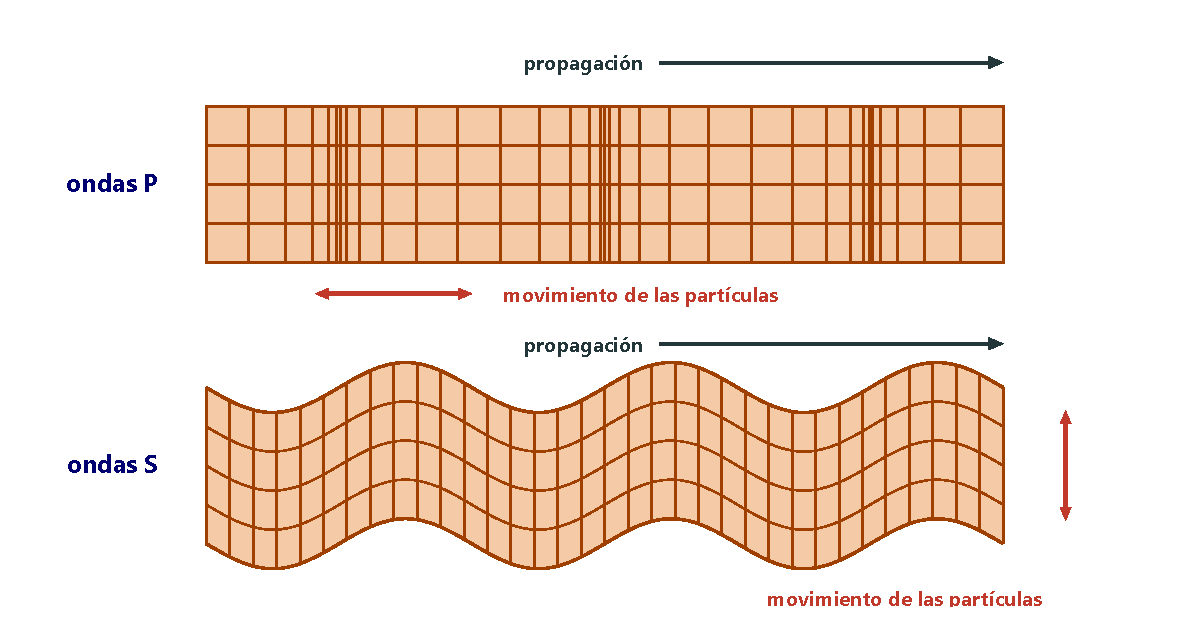
\includegraphics[width=0.7\textwidth]{images/UD13/ondas_sismicas}
    \caption{Ondas sísmicas P y S.}
    \label{fig:ondas_sismicas}
\end{figure}

\begin{exercise}
    En un terremoto se producen ondas sísmicas de dos tipos, P y S. Observa la figura~\ref{fig:ondas_sismicas} y clasifícalas en longitudinales y transversales.
    \begin{solu}
        Las ondas P son \textcolor{red}{longitudinales}: las partículas vibran en la misma dirección en que se propaga la onda (compresiones y dilataciones del terreno). Las ondas S son \textcolor{red}{transversales}: las partículas vibran perpendicularmente a la dirección de propagación.
    \end{solu}
\end{exercise}

%========================================================================================
\section{El sonido: una onda mecánica longitudinal}
%========================================================================================

Muchos animales, y también las personas, usamos el sonido para comunicarnos. Las cuerdas vocales o las cuerdas de un instrumento vibran, hacen vibrar el aire que las rodea y esa vibración llega hasta nuestros oídos. ¿Qué tipo de onda es el sonido?

\subsection{El sonido es un movimiento ondulatorio}

Si apoyas la mano sobre un altavoz mientras suena, notarás que su membrana vibra. Esas vibraciones empujan a las moléculas de aire cercanas, que empujan a su vez a las siguientes: por el aire se propagan zonas de mayor presión (\textbf{compresiones}) y de menor presión (\textbf{dilataciones}). El sonido tiene su origen en la \textbf{vibración de los cuerpos} y se \textbf{propaga} a través de un medio material.

\subsection{El sonido es una onda mecánica}

Si colocamos un timbre sonando dentro de una campana de vidrio conectada a una bomba de vacío, al principio se oye perfectamente. A medida que se extrae el aire, el sonido se debilita hasta que casi deja de oírse, aunque vemos que el martillo del timbre sigue golpeando. Si dejamos entrar de nuevo el aire, el sonido vuelve. El sonido \textbf{necesita un medio material} para propagarse: no se propaga en el vacío.

\begin{figure}[H]
    \centering
    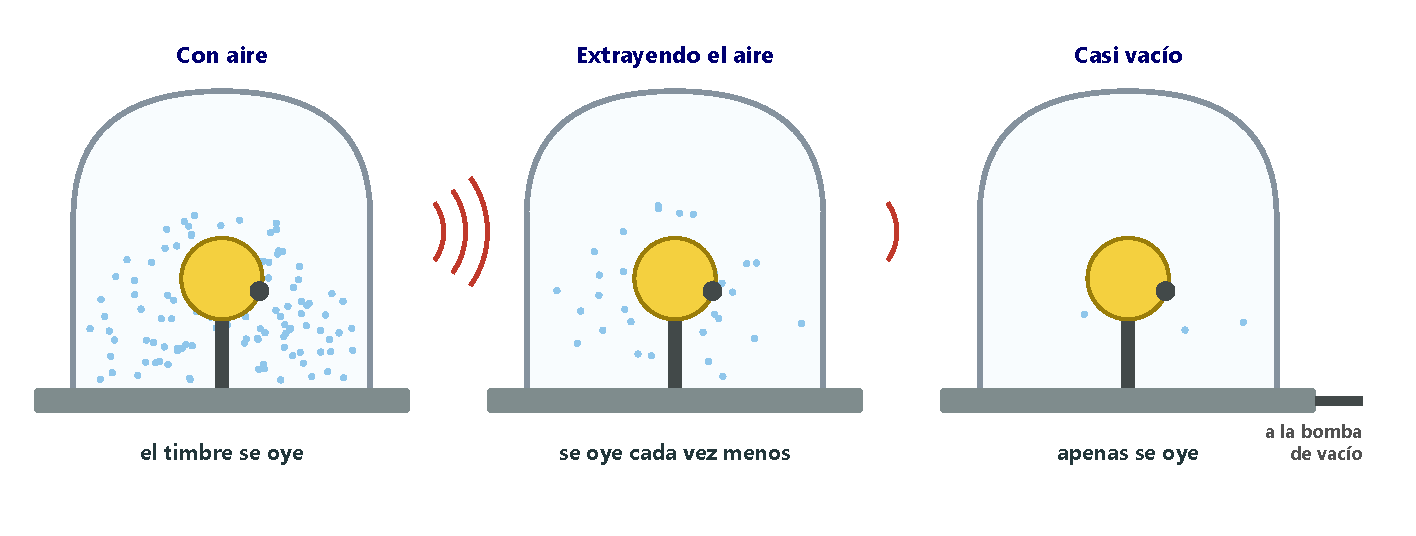
\includegraphics[width=0.85\textwidth]{images/UD13/campana_vacio}
    \caption{Un timbre en una campana de vacío: cuanto menos aire queda, menos se oye.}
    \label{fig:campana_vacio}
\end{figure}

\subsection{El sonido es una onda longitudinal}

Las moléculas de aire vibran hacia delante y hacia atrás en la \textbf{misma dirección} en que avanza el sonido: el sonido es una \textbf{onda longitudinal}. En un medio homogéneo se propaga con velocidad constante, es decir, con movimiento uniforme.

\begin{figure}[H]
    \centering
    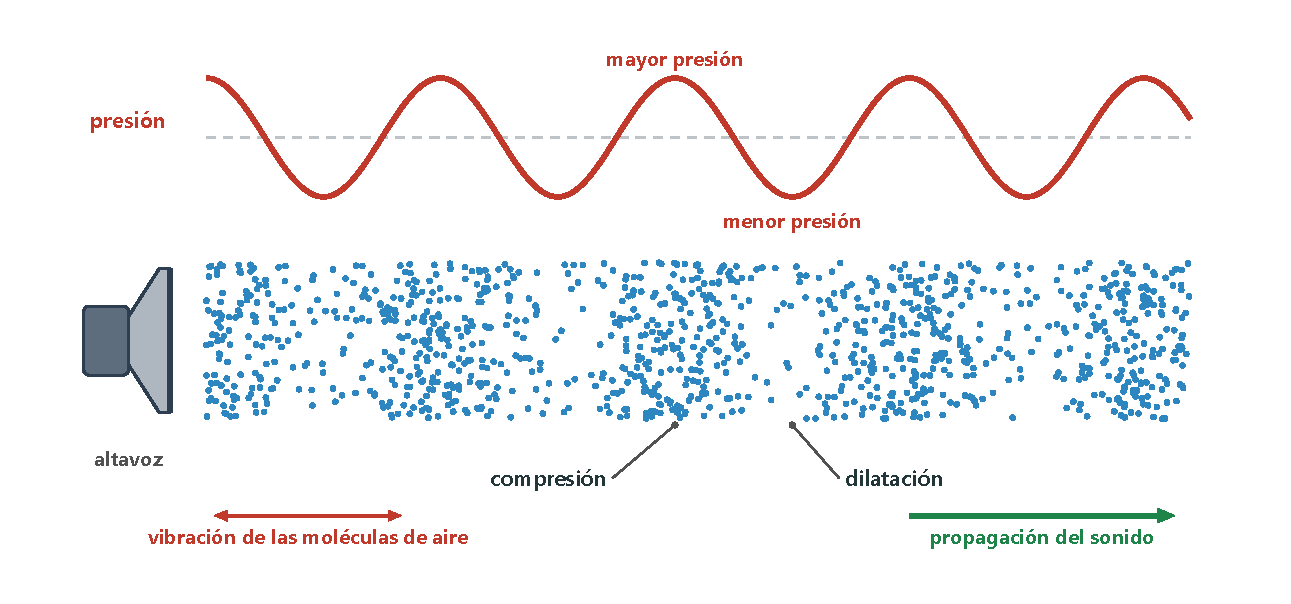
\includegraphics[width=0.9\textwidth]{images/UD13/sonido_compresiones}
    \caption{La membrana del altavoz produce compresiones y dilataciones del aire que se propagan en la misma dirección en que vibran las moléculas.}
    \label{fig:sonido_compresiones}
\end{figure}

La velocidad del sonido depende del medio: en general, es mayor en los sólidos que en los líquidos, y mayor en los líquidos que en los gases. En el aire, a unos \qty{15}{\degreeCelsius}, vale unos \qty{340}{\m\per\s}, y aumenta con la temperatura.

\begin{center}
    % --- tabla antigua ---
    % \begin{tblr}{colspec={lcccccccc}, hlines, vlines, row{1}={bg=ocre!85, fg=white, font=\bfseries}, column{1}={bg=ocre!85, fg=white, font=\bfseries}, cells={font=\small}}
        % Medio & vacío & aire & \ch{O2} & \ch{CO2} & agua & agua de mar & hierro & vidrio \\
        % \(v\) (\unit{\m\per\s}) & -- & 340 & 316 & 258 & 1450 & 1531 & 5100 & 5500 \\
    % \end{tblr}
    % --- tabla nueva ---
    {\small
    \begin{tabular}{@{}lcccccccc@{}}
        \toprule
        \textbf{Medio} & \textbf{vacío} & \textbf{aire} & \textbf{\ch{O2}} & \textbf{\ch{CO2}} & \textbf{agua} & \textbf{agua de mar} & \textbf{hierro} & \textbf{vidrio} \\
        \midrule
        \textbf{\(v\) (\unit{\m\per\s})} & -- & 340 & 316 & 258 & 1450 & 1531 & 5100 & 5500 \\
        \bottomrule
    \end{tabular}
    }
\end{center}

\begin{exercise}
    Observa la tabla anterior y compara la velocidad del sonido en los sólidos, los líquidos y los gases. ¿Por qué no aparece ningún valor en el vacío?
    \begin{solu}
        El sonido es \textcolor{red}{más rápido en los sólidos} (hierro y vidrio, más de \qty{5000}{\m\per\s}) que en los \textcolor{red}{líquidos} (agua, unos \qty{1500}{\m\per\s}), y en estos más que en los \textcolor{red}{gases} (aire, \ch{O2} y \ch{CO2}, unos \qty{300}{\m\per\s}). En el vacío \textcolor{red}{no se propaga}, porque es una onda mecánica.
    \end{solu}
\end{exercise}

\begin{exercise}
    Los ultrasonidos transportan mucha energía y pueden concentrarse en haces muy estrechos. Busca información sobre sus aplicaciones y prepara una breve presentación.
    \begin{solu}
        Respuesta libre. Por ejemplo: \textcolor{red}{ecografías} (seguimiento del embarazo, imágenes del corazón, hígado, riñones, tiroides\ldots), \textcolor{red}{sónar} para medir la profundidad del mar y localizar bancos de peces o submarinos, eliminación de cálculos renales, limpieza de piezas y joyas, detección de grietas en metales o ahuyentadores de animales.
    \end{solu}
\end{exercise}

\begin{example}
    Durante una tormenta vemos un relámpago y oímos el trueno \qty{3}{\s} después. ¿A qué distancia ha caído el rayo?

    La luz llega prácticamente al instante, así que el retraso se debe al sonido:
    \[ d = v \cdot t = \qty{340}{\m\per\s} \cdot \qty{3}{\s} = \textcolor{red}{\qty{1020}{\m}} \approx \qty{1}{\km} \]
\end{example}

\subsection{Intensidad física y nivel de intensidad sonora}

Como todas las ondas, el sonido transporta energía. Su \textbf{intensidad física}, \(I\), es la potencia que atraviesa cada unidad de superficie y, como hemos visto, a una distancia \(r\) de un foco que emite en todas las direcciones vale \(I = P/(4\pi r^2)\): \textbf{disminuye con el cuadrado de la distancia} al foco.

Sin embargo, nuestro oído no percibe la intensidad de forma proporcional. Por eso se usa el \textbf{nivel de intensidad sonora}, que se mide en \textbf{decibelios} (\unit{\decibel}):
\begin{itemize}
    \item El valor \qty{0}{\decibel} corresponde al \textbf{umbral de audición}, la intensidad mínima que puede percibir el oído humano.
    \item Cada vez que la intensidad física se hace \textbf{10 veces mayor}, el nivel de intensidad sonora \textbf{aumenta \qty{10}{\decibel}}. Si la intensidad se multiplica por 100, el nivel sube \qty{20}{\decibel}; si se multiplica por 1000, sube \qty{30}{\decibel}.
    \item El nivel máximo que el oído puede tolerar sin dolor es el \textbf{umbral del dolor}, de unos \qty{120}{\decibel}.
\end{itemize}

\begin{figure}[H]
    \centering
    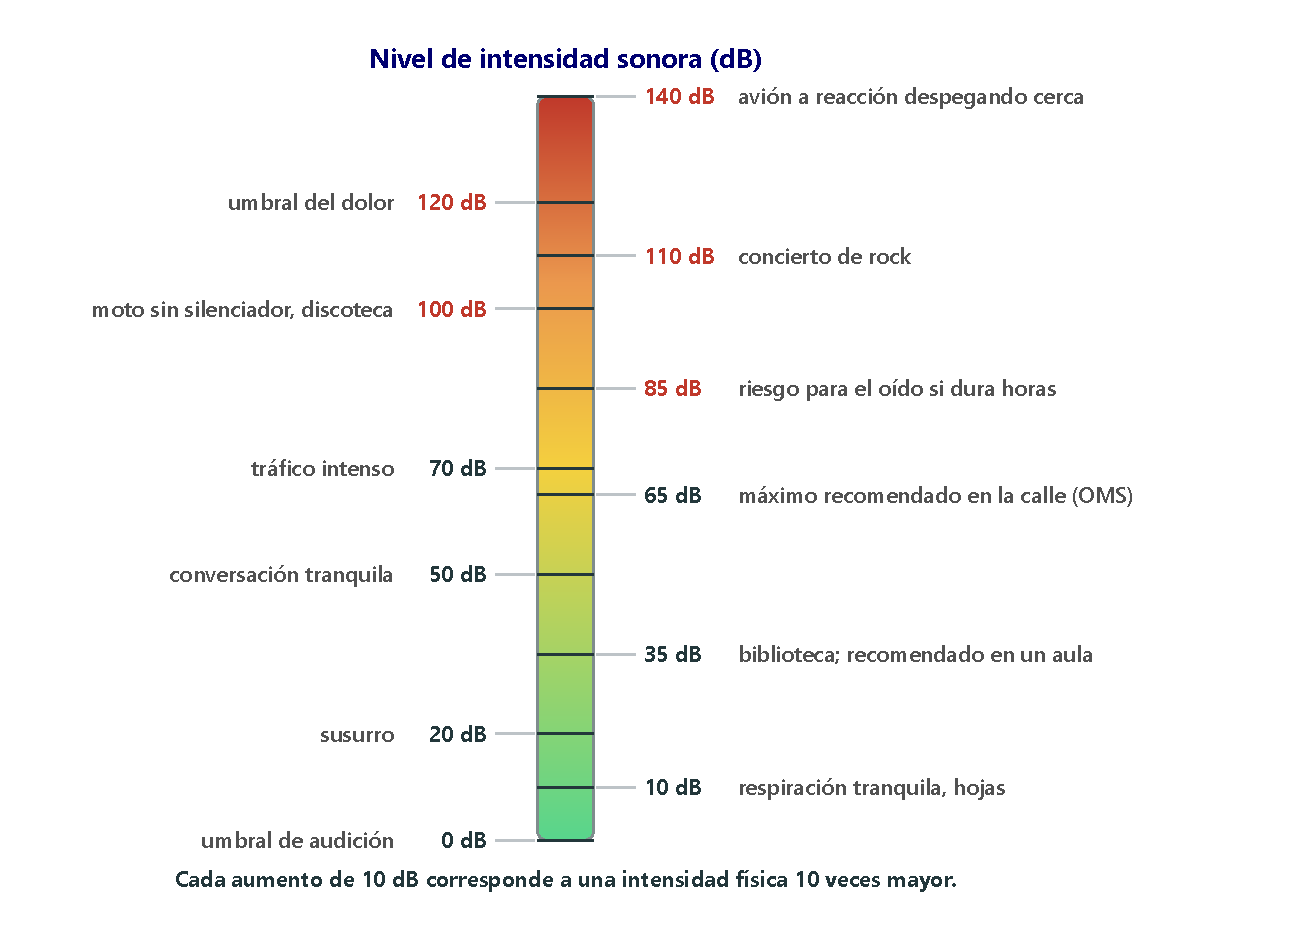
\includegraphics[width=0.95\textwidth]{images/UD13/escala_decibelios}
    \caption{Niveles de intensidad sonora de algunos sonidos habituales.}
    \label{fig:escala_decibelios}
\end{figure}

\begin{remark}
    Exponerse durante mucho tiempo a niveles superiores a unos \qty{85}{\decibel} (auriculares con el volumen alto, discotecas, conciertos) puede dañar el oído de forma permanente.
\end{remark}

\begin{example}
    Una conversación tiene un nivel de \qty{60}{\decibel}. ¿Qué nivel tendrá un sonido cuya intensidad física sea 1000 veces mayor?

    \(1000 = 10 \cdot 10 \cdot 10\): la intensidad se multiplica tres veces por 10, así que el nivel aumenta \(3 \cdot \qty{10}{\decibel}\):
    \[ \qty{60}{\decibel} + \qty{30}{\decibel} = \textcolor{red}{\qty{90}{\decibel}} \]
\end{example}

\subsection{¿Cómo se refleja el sonido? El eco}

Cuando las ondas sonoras encuentran un obstáculo, \textbf{se reflejan}. Si el sonido reflejado nos llega bastante después que el emitido, lo oímos como un sonido distinto: es el \textbf{eco}. Nuestro oído distingue dos sonidos si le llegan separados al menos \qty{0.1}{\s}. En ese tiempo el sonido recorre en el aire \(\qty{340}{\m\per\s} \cdot \qty{0.1}{\s} = \qty{34}{\m}\) de ida y vuelta, así que para percibir eco el obstáculo debe estar, como mínimo, a \textbf{\qty{17}{\m}}. Si está más cerca, el sonido reflejado se superpone al original y lo prolonga: es la \textbf{reverberación}.

El \textbf{sónar} de los barcos usa el eco de los ultrasonidos para medir la profundidad del mar: si el eco tarda un tiempo \(t\), el sonido ha recorrido dos veces la profundidad, \(2d = v \cdot t\).

\begin{figure}[H]
    \centering
    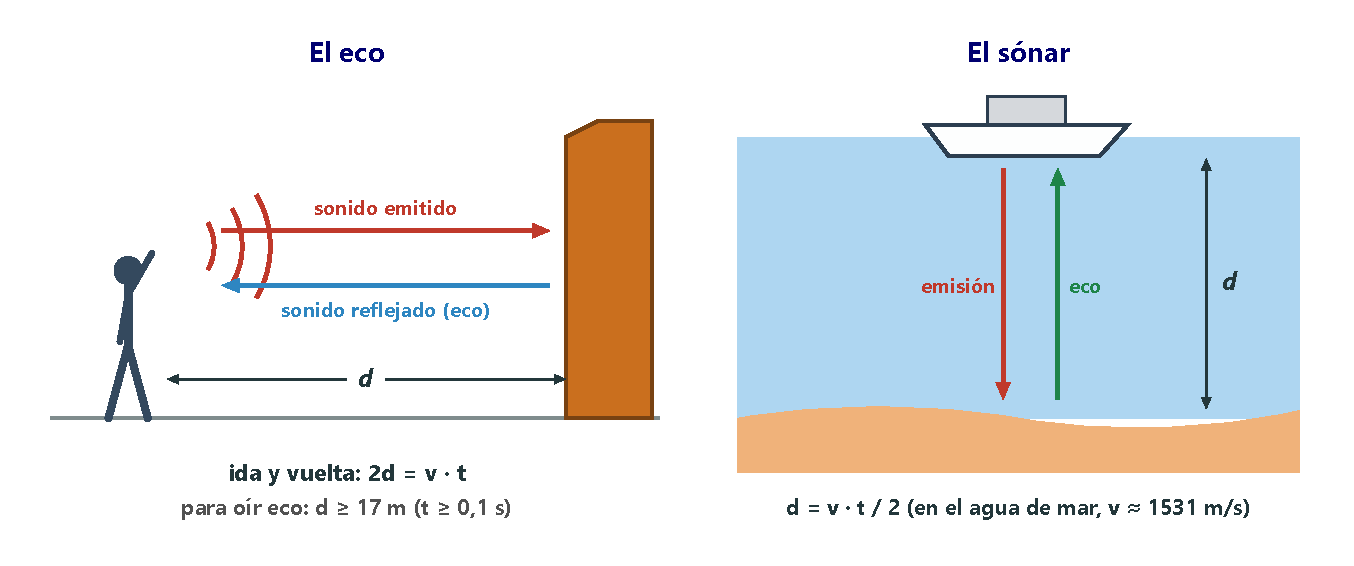
\includegraphics[width=0.95\textwidth]{images/UD13/eco_sonar}
    \caption{El eco y el sónar: el sonido recorre dos veces la distancia hasta el obstáculo.}
    \label{fig:eco_sonar}
\end{figure}

\begin{example}
    Gritamos frente a una pared rocosa y oímos el eco \qty{0.4}{\s} después. ¿A qué distancia está la pared?
    \[ 2d = v \cdot t \quad\Rightarrow\quad d = \frac{\qty{340}{\m\per\s} \cdot \qty{0.4}{\s}}{2} = \textcolor{red}{\qty{68}{\m}} \]
\end{example}

\subsection{¿Cómo se refracta el sonido?}

El sonido se refracta al pasar de un medio a otro y también al pasar de unas capas de aire a otras con distinta temperatura, porque en ellas se propaga con distinta velocidad. Por ejemplo, de noche el aire junto al mar está más frío que el de arriba; el sonido se curva hacia el agua y por eso, a veces, se oyen sonidos de la costa desde barcos muy alejados.

\subsection{¿Cuáles son las cualidades del sonido?}

\begin{itemize}
    \item \textbf{Intensidad}: permite distinguir los sonidos \textbf{fuertes} de los \textbf{débiles}. Depende de la \textbf{amplitud} de la onda: a mayor amplitud, sonido más fuerte.
    \item \textbf{Tono}: permite distinguir los sonidos \textbf{agudos} de los \textbf{graves}. Depende de la \textbf{frecuencia}: los sonidos agudos tienen \textbf{mayor} frecuencia que los graves. El oído humano solo percibe frecuencias entre \qty{20}{\hertz} y \qty{20000}{\hertz}; por debajo están los \textbf{infrasonidos} y por encima, los \textbf{ultrasonidos}.
    \item \textbf{Timbre}: permite distinguir dos sonidos de la misma intensidad y el mismo tono emitidos por focos distintos (por ejemplo, la misma nota tocada por una flauta y por un violín). Depende de la \textbf{forma de la onda}.
\end{itemize}

\begin{figure}[H]
    \centering
    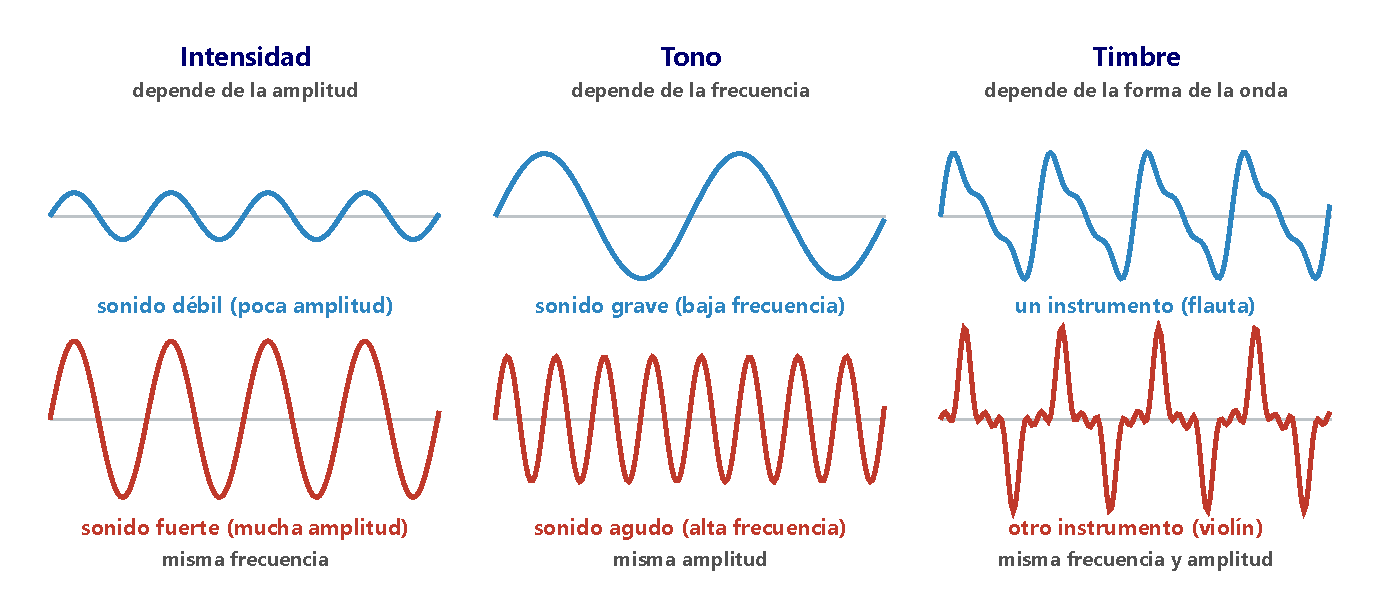
\includegraphics[width=\textwidth]{images/UD13/cualidades_sonido}
    \caption{Las cualidades del sonido dependen de la amplitud (intensidad), de la frecuencia (tono) y de la forma de la onda (timbre).}
    \label{fig:cualidades_sonido}
\end{figure}

\begin{exercise}
    Calcula entre qué valores está la longitud de onda de los sonidos audibles por las personas en el aire.
    \begin{solu}
        \(\lambda = v/f\). Para \qty{20}{\hertz}: \(\lambda = 340/20 = \textcolor{red}{\qty{17}{\m}}\). Para \qty{20000}{\hertz}: \(\lambda = 340/\num{20000} = \textcolor{red}{\qty{0.017}{\m}} = \qty{1.7}{\cm}\).
    \end{solu}
\end{exercise}

%----------------------------------------------------------------------------------------
\subsection*{Actividades de consolidación: el sonido}
%----------------------------------------------------------------------------------------

\begin{exercise}
    La velocidad del sonido en el aire aumenta con la temperatura, como muestra la tabla:
    \begin{center}
        % --- tabla antigua ---
        % \begin{tblr}{colspec={lcccccc}, hlines, vlines, column{1}={bg=ocre!85, fg=white, font=\bfseries}}
            % \(T\) (\unit{\degreeCelsius}) & \(-15\) & \(-10\) & \(-5\) & 0 & 5 & 10 \\
            % \(v\) (\unit{\m\per\s}) & 322 & 325 & 328 & 331 & 334 & 337 \\
        % \end{tblr}
        % --- tabla nueva ---
        \begin{tabular}{@{}lcccccc@{}}
            \toprule
            \textbf{\(T\) (\unit{\degreeCelsius})} & \(-15\) & \(-10\) & \(-5\) & 0 & 5 & 10 \\[3pt]
            \textbf{\(v\) (\unit{\m\per\s})} & 322 & 325 & 328 & 331 & 334 & 337 \\
            \bottomrule
        \end{tabular}
    \end{center}
    \begin{enumerate}[label=\alph*)]
        \item Representa la gráfica velocidad-temperatura. ¿Qué relación hay entre ambas magnitudes?
        \item ¿Qué le ocurrirá a un rayo sonoro que pasa de una zona de aire frío a otra más caliente?
        \item ¿Y si pasa de una zona caliente a otra más fría?
    \end{enumerate}
    \begin{solu}
        a) Los puntos están sobre una \textcolor{red}{recta}: la velocidad aumenta \qty{3}{\m\per\s} por cada \qty{5}{\degreeCelsius} (\qty{0.6}{\m\per\s} por grado). No es una proporcionalidad directa, porque a \qty{0}{\degreeCelsius} la velocidad no es cero.
        \begin{center}
            \begin{tikzpicture}
                \begin{axis}[grafica, xlabel={\(T\) (\unit{\degreeCelsius})}, ylabel={\(v\) (\unit{\m\per\s})}, xmin=-20, xmax=15, ymin=318, ymax=340]
                    \addplot coordinates {(-15,322) (-10,325) (-5,328) (0,331) (5,334) (10,337)};
                \end{axis}
            \end{tikzpicture}
        \end{center}
        b) Pasa a un medio en el que va más deprisa: el rayo \textcolor{red}{se aleja de la normal}.
        c) Pasa a un medio en el que va más despacio: el rayo \textcolor{red}{se acerca a la normal}.
    \end{solu}
\end{exercise}

\begin{exercise}
    Una soprano canta una nota de \qty{1300}{\hertz}. ¿Cuál es la longitud de onda de ese sonido en el aire si se propaga a \qty{332}{\m\per\s}?
    \begin{solu}
        \(\lambda = \dfrac{v}{f} = \dfrac{332}{1300} = \textcolor{red}{\qty{0.255}{\m}}\).
    \end{solu}
\end{exercise}

\begin{exercise}
    Una jueza de atletismo dispara la pistola de salida y oye el eco en una montaña \qty{2.5}{\s} después. ¿A qué distancia está la montaña? Dato: \(v_{\text{sonido}} = \qty{332}{\m\per\s}\).
    \begin{solu}
        El sonido va y vuelve: \(d = \dfrac{v \cdot t}{2} = \dfrac{332 \cdot \num{2.5}}{2} = \textcolor{red}{\qty{415}{\m}}\).
    \end{solu}
\end{exercise}

\begin{exercise}
    Una onda sonora pasa del aire al agua formando cierto ángulo con la normal. ¿Se acercará o se alejará de la normal? Justifícalo.
    \begin{solu}
        \textcolor{red}{Se alejará de la normal}, porque el sonido se propaga más deprisa en el agua (unos \qty{1450}{\m\per\s}) que en el aire (\qty{340}{\m\per\s}). (Al revés que la luz, que es más lenta en el agua.)
    \end{solu}
\end{exercise}

\begin{exercise}
    ¿Podríamos oír desde la Tierra el choque de un meteorito gigante contra la Luna? Razónalo.
    \begin{solu}
        \textcolor{red}{No}: entre la Luna y la Tierra el espacio está prácticamente vacío y el sonido, al ser una onda mecánica, no se propaga en el vacío. Sí podríamos \emph{ver} el destello, porque la luz se propaga en el vacío.
    \end{solu}
\end{exercise}

\begin{exercise}
    El sónar de un barco emite un pulso de ultrasonidos y recibe el eco del fondo \qty{0.52}{\s} después. ¿A qué profundidad está el fondo? Dato: \(v = \qty{1531}{\m\per\s}\).
    \begin{solu}
        \(d = \dfrac{v \cdot t}{2} = \dfrac{1531 \cdot \num{0.52}}{2} = 1531 \cdot \num{0.26} = \textcolor{red}{\qty{398}{\m}}\).
    \end{solu}
\end{exercise}

\begin{exercise}
    Estas dos gráficas representan dos sonidos de la misma frecuencia. ¿Cuál corresponde a un sonido fuerte y cuál a uno débil?
    \begin{center}
        \begin{tikzpicture}
            \begin{axis}[grafica, width=6.5cm, height=4cm, title={\small Sonido A}, xtick=\empty, ytick=\empty, xmin=0, xmax=3, ymin=-2.2, ymax=2.2, xlabel={tiempo}]
                \addplot[mark=none, samples=150, domain=0:3, blue!70!black] {0.5*sin(deg(2*pi*x))};
            \end{axis}
        \end{tikzpicture}\qquad
        \begin{tikzpicture}
            \begin{axis}[grafica, width=6.5cm, height=4cm, title={\small Sonido B}, xtick=\empty, ytick=\empty, xmin=0, xmax=3, ymin=-2.2, ymax=2.2, xlabel={tiempo}]
                \addplot[mark=none, samples=150, domain=0:3] {1.8*sin(deg(2*pi*x))};
            \end{axis}
        \end{tikzpicture}
    \end{center}
    \begin{solu}
        La intensidad depende de la amplitud: el sonido A, de poca amplitud, es \textcolor{red}{débil}, y el sonido B, de gran amplitud, es \textcolor{red}{fuerte}. Como tienen la misma frecuencia, tienen el mismo tono.
    \end{solu}
\end{exercise}

\begin{exercise}
    Un buque oceanográfico envía una señal de sónar hacia el fondo y la recibe \qty{0.1}{\s} después. ¿A qué profundidad está el fondo? Dato: \(v = \qty{1531}{\m\per\s}\).
    \begin{solu}
        \(d = \dfrac{1531 \cdot \num{0.1}}{2} = \textcolor{red}{\qty{76.6}{\m}}\).
    \end{solu}
\end{exercise}

\begin{exercise}
    Lee el texto y responde:
    \begin{marker}
        \emph{¿Por qué oímos a una soprano a pesar de la potencia de toda la orquesta? Al hablar y al cantar, producimos sonidos haciendo vibrar las cuerdas vocales: entre unos \qty{100}{\hertz} y \qty{220}{\hertz} en el habla normal, y entre \qty{50}{\hertz} y \qty{1500}{\hertz} en el canto. Una orquesta suena con más fuerza alrededor de los \qty{500}{\hertz}, y su sonido se debilita a frecuencias más altas. El oído humano es más sensible entre \qty{3000}{\hertz} y \qty{4000}{\hertz}, y muchas cantantes de ópera refuerzan su voz por encima de los \qty{2000}{\hertz}.}
    \end{marker}
    \begin{enumerate}[label=\alph*)]
        \item ¿Son audibles todas las frecuencias que aparecen en el texto?
        \item ¿A qué frecuencia suena con más fuerza una orquesta? ¿Para qué frecuencias es más sensible el oído?
        \item Calcula las longitudes de onda del habla normal y del canto (\(v = \qty{340}{\m\per\s}\)).
        \item ¿Por qué destaca la voz de la soprano sobre la orquesta?
    \end{enumerate}
    \begin{solu}
        a) \textcolor{red}{Sí}: todas están entre \qty{20}{\hertz} y \qty{20000}{\hertz}.
        b) La orquesta alcanza su máximo hacia los \textcolor{red}{\qty{500}{\hertz}}; el oído es más sensible entre \textcolor{red}{\qty{3000}{\hertz} y \qty{4000}{\hertz}}.
        c) Habla: \(\lambda = 340/100 = \qty{3.4}{\m}\) y \(\lambda = 340/220 = \qty{1.55}{\m}\), es decir, \textcolor{red}{entre \qty{1.55}{\m} y \qty{3.4}{\m}}. Canto: \(340/50 = \qty{6.8}{\m}\) y \(340/1500 = \qty{0.23}{\m}\), \textcolor{red}{entre \qty{0.23}{\m} y \qty{6.8}{\m}}.
        d) Porque la soprano concentra potencia en frecuencias \textcolor{red}{superiores a \qty{2000}{\hertz}}, donde la orquesta suena débil y donde el oído es más sensible.
    \end{solu}
\end{exercise}

\begin{exercise}
    Investiga cómo cambian los umbrales de audición y del dolor con la frecuencia:
    \begin{enumerate}[label=\alph*)]
        \item ¿Cuál es, aproximadamente, el umbral de audición para un sonido de \qty{512}{\hertz}?
        \item ¿Y el umbral del dolor para un sonido de \qty{4096}{\hertz}?
    \end{enumerate}
    \begin{solu}
        a) El umbral de audición depende mucho de la frecuencia (es más alto para los sonidos muy graves y muy agudos). A \qty{512}{\hertz} está en \textcolor{red}{unos pocos decibelios, menos de \qty{10}{\decibel}}.
        b) El umbral del dolor varía poco con la frecuencia: unos \textcolor{red}{\qty{120}{\decibel}}.
    \end{solu}
\end{exercise}

\begin{exercise}
    Un sonido tiene un nivel de intensidad de \qty{80}{\decibel}. ¿Qué nivel tendrá si su intensidad física se hace diez veces mayor? ¿Y cien veces mayor?
    \begin{solu}
        Diez veces mayor: \(80 + 10 = \textcolor{red}{\qty{90}{\decibel}}\). Cien veces mayor: \(80 + 20 = \textcolor{red}{\qty{100}{\decibel}}\).
    \end{solu}
\end{exercise}

\begin{exercise}
    Un avión emite un sonido con una potencia de \qty{3000}{\watt}. Calcula la intensidad física con la que se percibe: a) a \qty{1}{\km} del foco; b) a \qty{10}{\km} del foco.
    \begin{solu}
        a) \(I = \dfrac{P}{4\pi r^2} = \dfrac{3000}{4\pi \cdot (\num{1000})^2} = \textcolor{red}{\qty{2.39e-4}{\watt\per\square\m}}\).
        b) A una distancia 10 veces mayor, la intensidad es \(10^2 = 100\) veces menor: \(I = \textcolor{red}{\qty{2.39e-6}{\watt\per\square\m}}\).
    \end{solu}
\end{exercise}

%========================================================================================
\section{La luz: una onda transversal}
%========================================================================================

La luz es una \textbf{onda electromagnética}: se propaga en todas las direcciones desde un foco luminoso sin necesidad de un medio material. Por eso nos llega la luz del Sol y de las estrellas a través del espacio, que está prácticamente vacío. Todas las ondas electromagnéticas son \textbf{transversales}.

La luz se propaga en \textbf{línea recta} en un medio homogéneo; por eso los objetos opacos producen \textbf{sombras}. Su velocidad en el vacío es la mayor que existe:
\[ c = \qty{3e8}{\m\per\s} = \qty{300000}{\km\per\s} \]
En cualquier otro medio, la luz se propaga siempre más despacio.

\begin{example}
    La distancia media entre el Sol y la Tierra es de \qty{1.5e11}{\m}. ¿Cuánto tarda en llegarnos la luz del Sol?
    \[ t = \frac{d}{c} = \frac{\qty{1.5e11}{\m}}{\qty{3e8}{\m\per\s}} = \qty{500}{\s} = \textcolor{red}{\text{8 min 20 s}} \]
    Cuando miramos el Sol, lo vemos como era hace algo más de ocho minutos.
\end{example}

\subsection{¿Cómo se produce la reflexión de la luz?}

La \textbf{reflexión de la luz} es el cambio de dirección que experimenta un rayo luminoso al chocar con una superficie, por ejemplo un espejo, sin atravesarla. La luz reflejada sigue en el mismo medio y cumple las leyes de la reflexión que ya conocemos.

Un \textbf{espejo plano} es una superficie plana, lisa y pulida, que refleja en una sola dirección un haz de rayos paralelos. Para encontrar la imagen de un punto \(P\) de un objeto, trazamos dos rayos que salen de \(P\) y se reflejan en el espejo. Los rayos reflejados se separan, pero sus \textbf{prolongaciones} (hacia detrás del espejo) se cortan en un punto \(P'\): es la imagen de \(P\).

\begin{figure}[H]
    \centering
    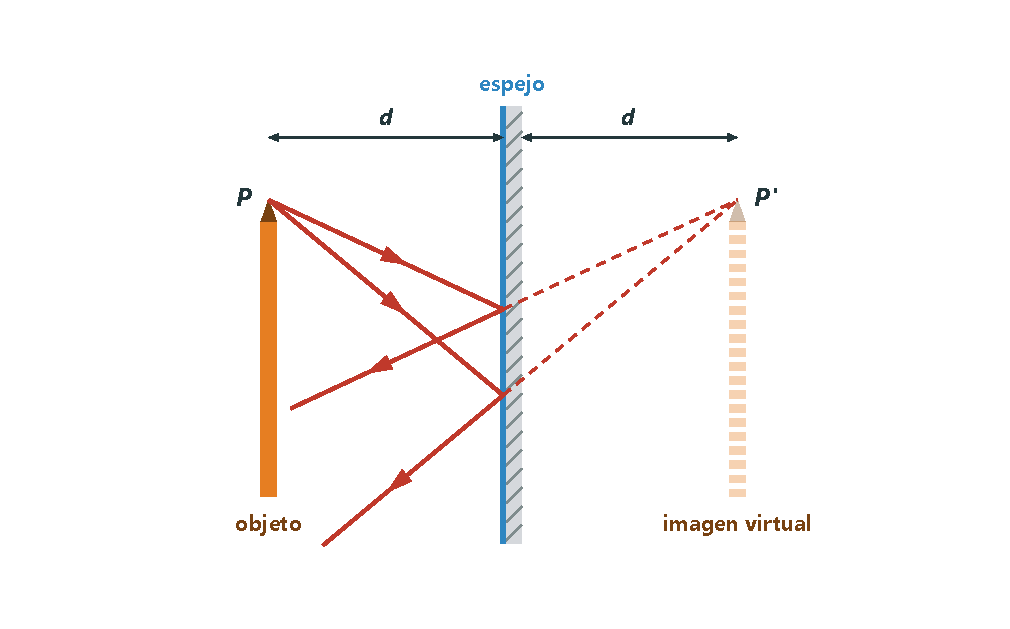
\includegraphics[width=0.65\textwidth]{images/UD13/espejo_plano}
    \caption{Formación de la imagen en un espejo plano: las prolongaciones de los rayos reflejados se cortan detrás del espejo.}
    \label{fig:espejo_plano}
\end{figure}

\begin{marker}
    La imagen en un espejo plano es \textbf{virtual} (se forma con las prolongaciones de los rayos, no con los rayos mismos, y no se puede recoger en una pantalla), \textbf{del mismo tamaño} que el objeto, \textbf{derecha}, está \textbf{a la misma distancia} del espejo que el objeto y tiene \textbf{invertidos la izquierda y la derecha}.
\end{marker}

\subsection{¿Cómo se produce la refracción de la luz?}

La \textbf{refracción de la luz} es el cambio de velocidad, y en general de dirección, que experimenta un rayo de luz al pasar de un medio a otro en el que se propaga con distinta velocidad.

\begin{definition}[Índice de refracción]
    El \textbf{índice de refracción}, \(n\), de un medio es el cociente entre la velocidad de la luz en el vacío, \(c\), y su velocidad en ese medio, \(v\):
    \[ n = \frac{c}{v} \]
    No tiene unidades, porque es el cociente de dos velocidades. Como la luz nunca es más rápida que en el vacío, \(n \geq 1\).
\end{definition}

\begin{center}
    % --- tabla antigua ---
    % \begin{tblr}{colspec={lccccccc}, hlines, vlines, row{1}={bg=ocre!85, fg=white, font=\bfseries}, column{1}={bg=ocre!85, fg=white, font=\bfseries}, cells={font=\small}}
        % Medio & vacío & aire & agua & alcohol & cuarzo & vidrio & diamante \\
        % \(n\) & 1 & \num{1.0003} & \num{1.33} & \num{1.36} & \num{1.46} & \num{1.5} & \num{2.42} \\
    % \end{tblr}
    % --- tabla nueva ---
    {\small
    \begin{tabular}{@{}lccccccc@{}}
        \toprule
        \textbf{Medio} & \textbf{vacío} & \textbf{aire} & \textbf{agua} & \textbf{alcohol} & \textbf{cuarzo} & \textbf{vidrio} & \textbf{diamante} \\
        \midrule
        \textbf{\(n\)} & 1 & \num{1.0003} & \num{1.33} & \num{1.36} & \num{1.46} & \num{1.5} & \num{2.42} \\
        \bottomrule
    \end{tabular}
    }
\end{center}

Cuanto mayor es el índice de refracción, más despacio va la luz por ese medio y decimos que el medio es más \textbf{refringente}. Por eso, cuando la luz pasa de un medio a otro de \textbf{mayor} índice (del aire al agua), el rayo \textbf{se acerca a la normal}; y cuando pasa a uno de \textbf{menor} índice (del agua al aire), \textbf{se aleja de la normal}.

La \textbf{ley de Snell} de la refracción establece que el cociente entre el seno del ángulo de incidencia y el del ángulo de refracción es constante, e igual al cociente entre las velocidades de la luz en los dos medios:
\begin{equation*}
    \boxed{\frac{\sen i}{\sen r} = \frac{v_1}{v_2} = \frac{n_2}{n_1}}
\end{equation*}

\begin{figure}[H]
    \centering
    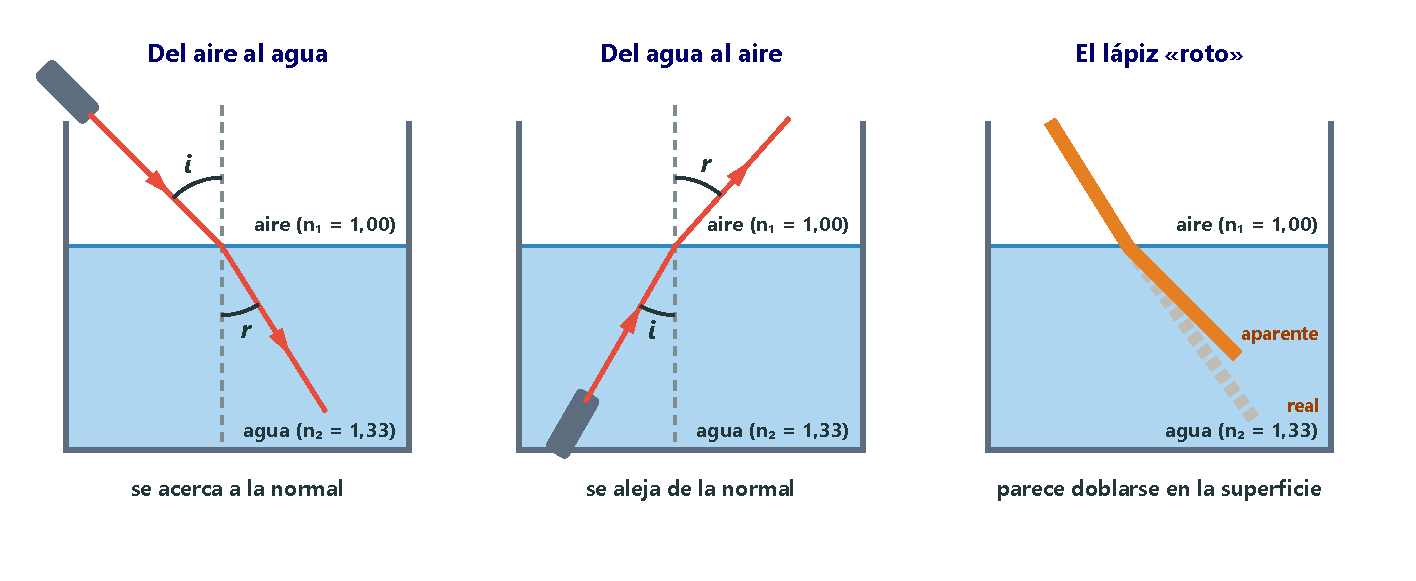
\includegraphics[width=\textwidth]{images/UD13/refraccion_luz}
    \caption{Refracción de un rayo láser al pasar del aire al agua y del agua al aire. La refracción explica que un lápiz parezca doblado al meterlo en agua.}
    \label{fig:refraccion_luz}
\end{figure}

\begin{example}
    Un rayo de luz pasa del aire (\(n_1 = 1\)) al agua (\(n_2 = \num{1.33}\)) con un ángulo de incidencia de \ang{30}. Calcula la velocidad de la luz en el agua y el ángulo de refracción.
    \[ v = \frac{c}{n} = \frac{\qty{3e8}{\m\per\s}}{\num{1.33}} = \textcolor{red}{\qty{2.26e8}{\m\per\s}} \]
    \[ \sen r = \frac{n_1 \cdot \sen i}{n_2} = \frac{1 \cdot \sen \ang{30}}{\num{1.33}} = \frac{\num{0.5}}{\num{1.33}} = \num{0.376} \quad\Rightarrow\quad r = \textcolor{red}{\ang{22.1}} \]
    El rayo se acerca a la normal (\(r < i\)), porque la luz es más lenta en el agua.
\end{example}

\begin{exercise}
    El índice de refracción de un vidrio es \num{1.5}. ¿A qué velocidad se propaga la luz en él?
    \begin{solu}
        \(v = \dfrac{c}{n} = \dfrac{\num{3e8}}{\num{1.5}} = \textcolor{red}{\qty{2e8}{\m\per\s}}\).
    \end{solu}
\end{exercise}

%----------------------------------------------------------------------------------------
\subsection*{Actividades de consolidación: la luz}
%----------------------------------------------------------------------------------------

\begin{exercise}
    Lee el texto y responde:
    \begin{marker}
        \emph{En lo que respecta a la luz, las ondas se parecen a las del sonido: son tridimensionales y tienen una frecuencia, una longitud de onda y una velocidad (en este caso, la de la luz). Pero, sorprendentemente, no necesitan un medio como el aire para propagarse: la luz del Sol y de las estrellas nos llega aunque tenga que atravesar el espacio, que es un vacío casi perfecto. La frecuencia de la luz visible es altísima: cada segundo llegan a nuestros ojos unos 600 billones de ondas.} (Adaptado de Carl Sagan.)
    \end{marker}
    \begin{enumerate}[label=\alph*)]
        \item Según el texto, ¿en qué se diferencian las ondas de luz y las de sonido?
        \item Añade otra diferencia entre ambas.
        \item ¿Qué tienen en común?
        \item Calcula la longitud de onda de una luz de 600 billones de hercios.
        \item Si la luz tarda \qty{1.3}{\s} en llegar de la Luna a la Tierra, ¿a qué distancia está la Luna?
    \end{enumerate}
    \begin{solu}
        a) La luz \textcolor{red}{no necesita un medio material} (es una onda electromagnética) y el sonido sí (es una onda mecánica).
        b) La luz es \textcolor{red}{transversal} y el sonido, longitudinal. Además, la luz es muchísimo más rápida.
        c) Las dos son ondas que \textcolor{red}{transportan energía} sin transportar materia, se propagan en las tres dimensiones y tienen frecuencia, longitud de onda y velocidad; las dos se reflejan y se refractan.
        d) \(f = \qty{6e14}{\hertz}\); \(\lambda = \dfrac{c}{f} = \dfrac{\num{3e8}}{\num{6e14}} = \textcolor{red}{\qty{5e-7}{\m}} = \qty{500}{\nano\m}\) (luz verde-azulada).
        e) \(d = c \cdot t = \num{3e8} \cdot \num{1.3} = \textcolor{red}{\qty{3.9e8}{\m}}\), unos \qty{390000}{\km}. (La distancia media real es de unos \qty{384000}{\km}: la luz tarda unos \qty{1.28}{\s}.)
    \end{solu}
\end{exercise}

\begin{exercise}
    Copia el esquema en tu cuaderno e identifica: a) el medio 1 y el medio 2; b) la superficie de separación; c) la normal; d) los ángulos de incidencia, de reflexión y de refracción.
    \begin{center}
        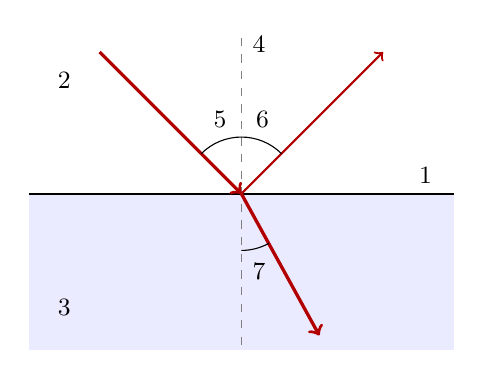
\begin{tikzpicture}[scale=0.9]
            \fill[blue!8] (-3,0) rectangle (3,-2.2);
            \draw[thick] (-3,0) -- (3,0);
            \draw[dashed, gray] (0,2.2) -- (0,-2.2);
            \draw[very thick, red!70!black, ->] (-2,2) -- (0,0);
            \draw[thick, red!70!black, ->] (0,0) -- (2,2);
            \draw[very thick, red!70!black, ->] (0,0) -- (1.1,-2);
            \node[above] at (2.6,0) {\small 1};
            \node at (-2.5,1.6) {\small 2};
            \node at (-2.5,-1.6) {\small 3};
            \node at (0.25,2.1) {\small 4};
            \draw (0,0.8) arc (90:135:0.8); \node at (-0.3,1.05) {\small 5};
            \draw (0,0.8) arc (90:45:0.8); \node at (0.3,1.05) {\small 6};
            \draw (0,-0.8) arc (270:299:0.8); \node at (0.25,-1.1) {\small 7};
        \end{tikzpicture}
    \end{center}
    \begin{solu}
        a) \textcolor{red}{2} es el medio 1 (por donde llega el rayo) y \textcolor{red}{3} es el medio 2. b) La superficie de separación es la línea horizontal (\textcolor{red}{1}). c) La normal es la línea discontinua (\textcolor{red}{4}). d) \textcolor{red}{5} es el ángulo de incidencia, \textcolor{red}{6} el de reflexión (igual que el de incidencia) y \textcolor{red}{7} el de refracción (menor: el medio 2 es más refringente).
    \end{solu}
\end{exercise}

\begin{exercise}
    Con un montaje como el de la figura~\ref{fig:refraccion_luz}, un láser pasa del aire al vidrio. Se han medido estos ángulos:
    \begin{center}
        % --- tabla antigua ---
        % \begin{tblr}{colspec={ccccc}, hlines, vlines, row{1}={bg=ocre!85, fg=white, font=\bfseries}}
            % Incidencia & Refracción & \(\sen i\) & \(\sen r\) & \(\sen i / \sen r\) \\
            % \ang{15} & \ang{9.43} & \num{0.259} & \num{0.164} & \ldots \\
            % \ang{30} & \ang{18.40} & \num{0.500} & \num{0.316} & \ldots \\
            % \ang{45} & \ang{26.60} & \num{0.707} & \num{0.448} & \ldots \\
        % \end{tblr}
        % --- tabla nueva ---
        \begin{tabular}{@{}ccccc@{}}
            \toprule
            \textbf{Incidencia} & \textbf{Refracción} & \textbf{\(\sen i\)} & \textbf{\(\sen r\)} & \textbf{\(\sen i / \sen r\)} \\
            \midrule
            \ang{15} & \ang{9.43} & \num{0.259} & \num{0.164} & \ldots \\[3pt]
            \ang{30} & \ang{18.40} & \num{0.500} & \num{0.316} & \ldots \\[3pt]
            \ang{45} & \ang{26.60} & \num{0.707} & \num{0.448} & \ldots \\
            \bottomrule
        \end{tabular}
    \end{center}
    \begin{enumerate}[label=\alph*)]
        \item Completa la última columna.
        \item ¿Cómo es ese cociente? ¿Qué relación guarda con la velocidad de la luz en los dos medios?
        \item ¿Qué ocurre si el ángulo de incidencia es \ang{0}?
    \end{enumerate}
    \begin{solu}
        a) \(\num{0.259}/\num{0.164} = \num{1.58}\); \(\num{0.500}/\num{0.316} = \num{1.58}\); \(\num{0.707}/\num{0.448} = \num{1.58}\).
        b) Es \textcolor{red}{constante} (\(\approx \num{1.58}\)): es el cociente \(v_{\text{aire}}/v_{\text{vidrio}}\), que coincide con el índice de refracción del vidrio. La luz va \num{1.58} veces más despacio en este vidrio.
        c) El rayo entra en el vidrio \textcolor{red}{sin desviarse}.
    \end{solu}
\end{exercise}

\begin{exercise}
    Repetimos la experiencia anterior sustituyendo el vidrio por agua y obtenemos:
    \begin{center}
        % --- tabla antigua ---
        % \begin{tblr}{colspec={ccccc}, hlines, vlines, row{1}={bg=ocre!85, fg=white, font=\bfseries}}
            % Incidencia & Refracción & \(\sen i\) & \(\sen r\) & \(\sen i / \sen r\) \\
            % \ang{15} & \ang{11.23} & \num{0.259} & \num{0.195} & \ldots \\
            % \ang{30} & \ang{22.00} & \num{0.500} & \num{0.375} & \ldots \\
            % \ang{45} & \ang{32.00} & \num{0.707} & \num{0.530} & \ldots \\
        % \end{tblr}
        % --- tabla nueva ---
        \begin{tabular}{@{}ccccc@{}}
            \toprule
            \textbf{Incidencia} & \textbf{Refracción} & \textbf{\(\sen i\)} & \textbf{\(\sen r\)} & \textbf{\(\sen i / \sen r\)} \\
            \midrule
            \ang{15} & \ang{11.23} & \num{0.259} & \num{0.195} & \ldots \\[3pt]
            \ang{30} & \ang{22.00} & \num{0.500} & \num{0.375} & \ldots \\[3pt]
            \ang{45} & \ang{32.00} & \num{0.707} & \num{0.530} & \ldots \\
            \bottomrule
        \end{tabular}
    \end{center}
    \begin{enumerate}[label=\alph*)]
        \item Completa la última columna.
        \item Compara con la actividad anterior. ¿Qué ley de la refracción puedes enunciar?
        \item Explica por qué una pajita metida en un vaso de agua parece doblada.
    \end{enumerate}
    \begin{solu}
        a) \(\num{1.33}\) en los tres casos (\num{1.328}, \num{1.333} y \num{1.334}).
        b) Para el mismo ángulo de incidencia, los ángulos de refracción son \textcolor{red}{mayores} que en el vidrio: el agua es menos refringente. En los dos casos, \textcolor{red}{el cociente \(\sen i / \sen r\) es constante} para cada par de medios (ley de Snell) e igual al índice de refracción del segundo medio respecto del aire.
        c) La luz que sale de la parte sumergida pasa del agua al aire y \textcolor{red}{se aleja de la normal}. Nuestro cerebro prolonga los rayos en línea recta y «ve» la parte sumergida más arriba de donde está: la pajita parece quebrada en la superficie.
    \end{solu}
\end{exercise}

\begin{exercise}
    En un espejo plano, el rayo incidente y el reflejado forman entre sí un ángulo de \ang{100}. ¿Qué ángulo forma el rayo incidente con la superficie del espejo?
    \begin{solu}
        Cada rayo forma con la normal \(\ang{100}/2 = \ang{50}\). Con la superficie: \(\ang{90} - \ang{50} = \textcolor{red}{\ang{40}}\).
    \end{solu}
\end{exercise}

\begin{exercise}
    Calcula la velocidad de la luz en el agua (\(n = \num{1.33}\)), en el cuarzo (\(n = \num{1.46}\)) y en el diamante (\(n = \num{2.42}\)). Dato: \(c = \qty{3e8}{\m\per\s}\).
    \begin{solu}
        \(v = c/n\): agua, \(\textcolor{red}{\qty{2.26e8}{\m\per\s}}\); cuarzo, \(\textcolor{red}{\qty{2.05e8}{\m\per\s}}\); diamante, \(\textcolor{red}{\qty{1.24e8}{\m\per\s}}\).
    \end{solu}
\end{exercise}

\begin{exercise}
    ¿Puede una sustancia tener un índice de refracción de \num{0.9}? Justifícalo.
    \begin{solu}
        \textcolor{red}{No}: si \(n = c/v = \num{0.9}\), la luz iría por ese medio más deprisa que por el vacío (\(v = c/\num{0.9} \approx \num{1.11}\,c\)), y la velocidad de la luz en el vacío es la máxima posible.
    \end{solu}
\end{exercise}

\begin{exercise}
    ¿Con qué ángulo debe incidir un rayo de luz sobre un espejo para que el rayo incidente y el reflejado sean perpendiculares?
    \begin{solu}
        Entre los dos deben sumar \ang{90} y son iguales: \(i = \textcolor{red}{\ang{45}}\).
    \end{solu}
\end{exercise}

\begin{exercise}
    Un rayo de luz pasa del agua (\(n = \num{1.33}\)) al aire (\(n = 1\)) y el rayo refractado sale rasante, formando \ang{90} con la normal. ¿Cuál era el ángulo de incidencia?
    \begin{solu}
        \(n_1 \sen i = n_2 \sen r \Rightarrow \num{1.33} \cdot \sen i = 1 \cdot \sen \ang{90} = 1\). \(\sen i = \dfrac{1}{\num{1.33}} = \num{0.752}\), \(i = \textcolor{red}{\ang{48.8}}\). (Si el ángulo de incidencia es mayor, la luz no sale del agua: se refleja por completo. Es la \emph{reflexión total}, en la que se basa la fibra óptica.)
    \end{solu}
\end{exercise}

\begin{exercise}
    ¿Por qué no somos capaces de leer un cartel reflejado en un espejo?
    \begin{solu}
        Porque la imagen de un espejo plano tiene \textcolor{red}{invertidas la izquierda y la derecha}: las letras aparecen al revés y el texto se lee de derecha a izquierda. Por eso en las ambulancias se escribe «AMBULANCIA» al revés: así se lee bien en el retrovisor.
    \end{solu}
\end{exercise}

\begin{exercise}
    Escribe tu nombre tal y como se vería reflejado en un espejo y compruébalo.
    \begin{solu}
        Respuesta libre. Hay que escribir las letras de derecha a izquierda y cada una invertida.
    \end{solu}
\end{exercise}

%========================================================================================
\section{El espectro electromagnético}
%========================================================================================

\subsection{La dispersión de la luz blanca}

Un \textbf{prisma óptico} es un cuerpo transparente, homogéneo e isótropo, limitado por caras planas no paralelas, cuyo índice de refracción es mayor que el del aire. Cuando un rayo de luz de un solo color llega a una de sus caras, se refracta acercándose a la normal; al salir por la otra cara, vuelve a refractarse alejándose de ella. En total, el rayo se desvía.

La \textbf{luz blanca} es una mezcla de radiaciones de distintos colores (distintas longitudes de onda). Dentro del vidrio, cada color se propaga con una velocidad ligeramente distinta, así que cada uno se refracta con un ángulo diferente: el violeta es el que más se desvía y el rojo, el que menos. Al salir del prisma, los colores se separan. Este fenómeno se llama \textbf{dispersión} de la luz, y la banda de colores que se obtiene es el \textbf{espectro visible} de la luz blanca. El arcoíris es un ejemplo natural: las gotas de lluvia actúan como pequeños prismas.

\begin{figure}[H]
    \centering
    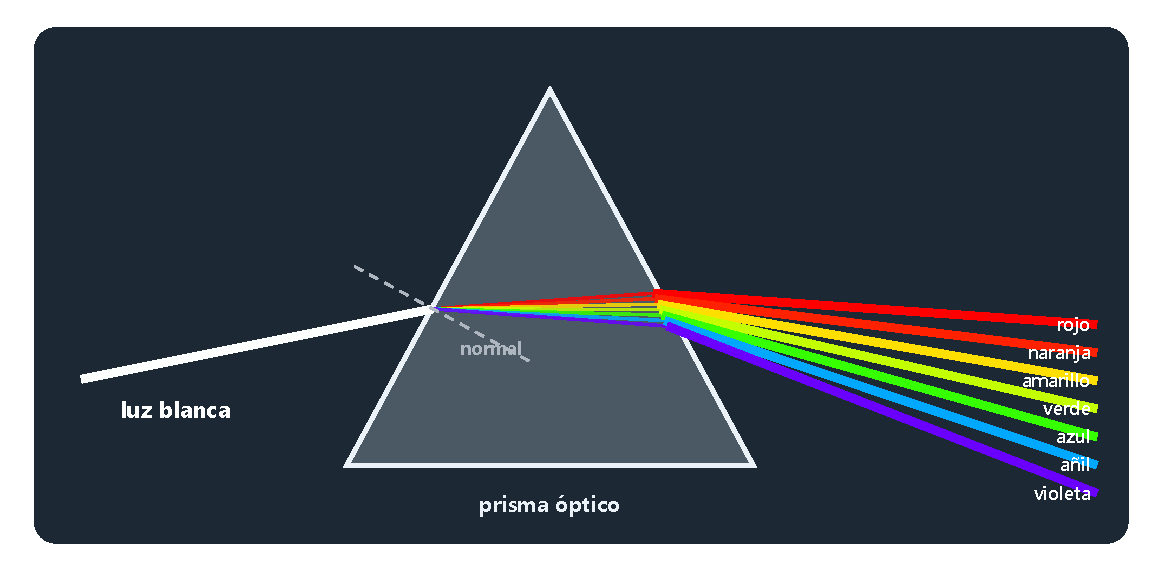
\includegraphics[width=0.75\textwidth]{images/UD13/prisma}
    \caption{Dispersión de la luz blanca en un prisma óptico.}
    \label{fig:prisma}
\end{figure}

\subsection{El espectro electromagnético y sus aplicaciones}

La luz visible es solo una pequeña parte de un conjunto mucho más amplio de ondas, el \textbf{espectro electromagnético}. Todas son ondas electromagnéticas, se propagan en el vacío a \qty{3e8}{\m\per\s} y cumplen \(c = \lambda \cdot f\); se diferencian en su frecuencia y su longitud de onda. Cuanto mayor es la frecuencia, \textbf{mayor es la energía} que transporta la radiación.

\begin{figure}[H]
    \centering
    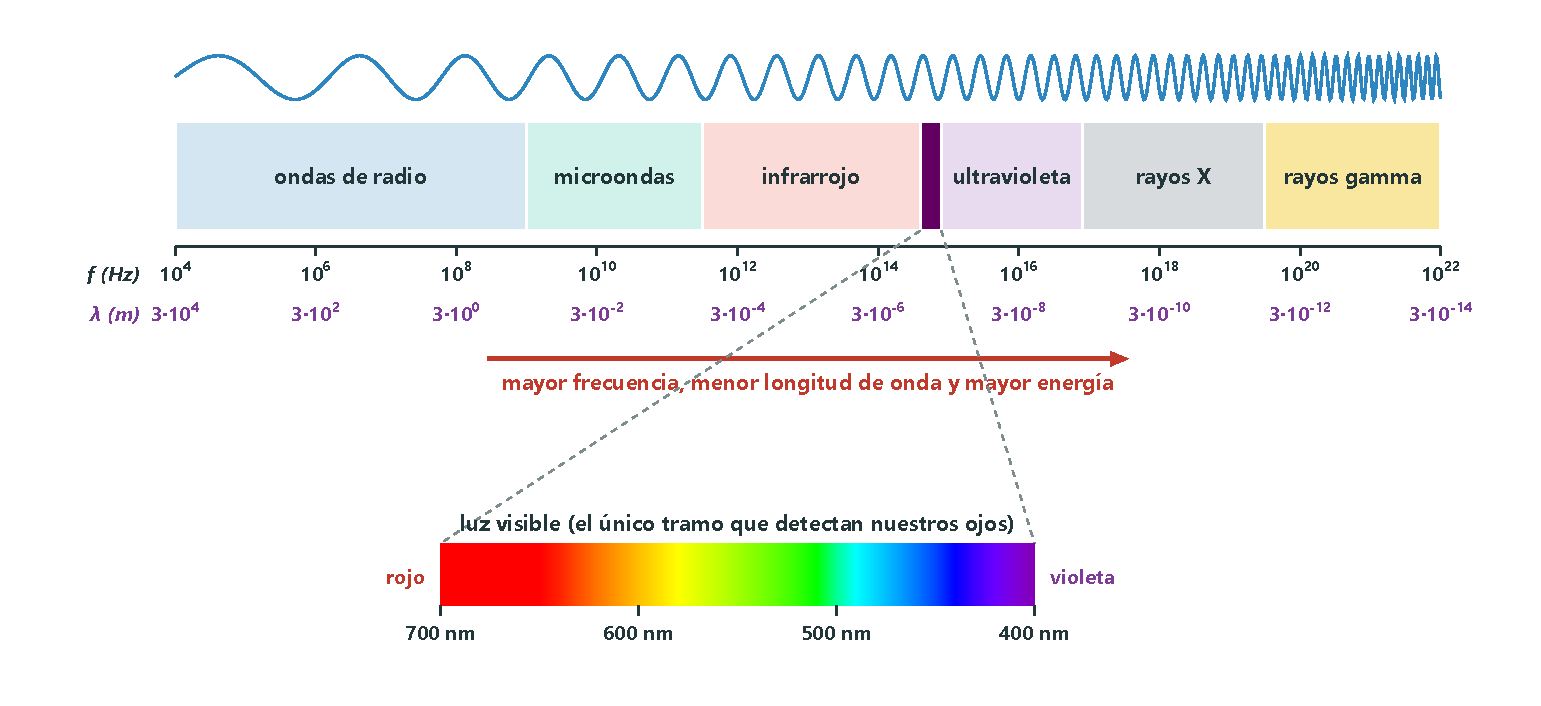
\includegraphics[width=\textwidth]{images/UD13/espectro_em}
    \caption{El espectro electromagnético. La luz visible ocupa un tramo muy estrecho, entre unos \qty{700}{\nano\m} (rojo) y \qty{400}{\nano\m} (violeta).}
    \label{fig:espectro_em}
\end{figure}

\begin{center}
    % --- tabla antigua ---
    % \begin{tblr}{colspec={Q[l,3.2cm]X}, width=\linewidth, hlines, vlines, row{1}={bg=ocre!85, fg=white, font=\bfseries}, column{1}={font=\bfseries}, cells={font=\small}}
        % Radiación & Algunas aplicaciones \\
        % Ondas de radio & Radio y televisión, comunicaciones. Los radiotelescopios captan las ondas de radio que emiten algunas estrellas y galaxias. \\
        % Microondas & Radar (detección de barcos y aviones, control de velocidad), telefonía móvil, wifi, comunicaciones por satélite y hornos de microondas, en los que el agua de los alimentos absorbe la radiación y se calienta. \\
        % Infrarrojos & Los emite cualquier cuerpo caliente (también nuestro cuerpo). Mandos a distancia, cámaras de visión nocturna y termografía, que detecta zonas del cuerpo con una temperatura anormal (inflamaciones, algunos tumores, lesiones deportivas). \\
        % Luz visible & Visión, iluminación, fotosíntesis, láser, fibra óptica. \\
        % Ultravioleta & Broncean y queman la piel, que se oscurece para defenderse. Se usan como desinfectante (esterilización) y para detectar rastros biológicos o billetes y obras de arte falsificados. \\
        % Rayos X & Atraviesan con facilidad los tejidos blandos, pero no los huesos: radiografías y tomografía axial computarizada (TAC), que crea imágenes en 3D de los órganos. \\
        % Rayos gamma & Los emiten las sustancias radiactivas; tienen muchísima energía. Medicina nuclear (gammagrafías, diagnóstico de tumores) y radiocirugía con «bisturí de rayos gamma» para tratar tumores en zonas delicadas. \\
    % \end{tblr}
    % --- tabla nueva ---
    {\small
    \begin{tabular}{@{}L{3.2cm} p{0.78\linewidth}@{}}
        \toprule
        \textbf{Radiación} & \textbf{Algunas aplicaciones} \\
        \midrule
        \textbf{Ondas de radio} & Radio y televisión, comunicaciones. Los radiotelescopios captan las ondas de radio que emiten algunas estrellas y galaxias. \\[3pt]
        \textbf{Microondas} & Radar (detección de barcos y aviones, control de velocidad), telefonía móvil, wifi, comunicaciones por satélite y hornos de microondas, en los que el agua de los alimentos absorbe la radiación y se calienta. \\[3pt]
        \textbf{Infrarrojos} & Los emite cualquier cuerpo caliente (también nuestro cuerpo). Mandos a distancia, cámaras de visión nocturna y termografía, que detecta zonas del cuerpo con una temperatura anormal (inflamaciones, algunos tumores, lesiones deportivas). \\[3pt]
        \textbf{Luz visible} & Visión, iluminación, fotosíntesis, láser, fibra óptica. \\[3pt]
        \textbf{Ultravioleta} & Broncean y queman la piel, que se oscurece para defenderse. Se usan como desinfectante (esterilización) y para detectar rastros biológicos o billetes y obras de arte falsificados. \\[3pt]
        \textbf{Rayos X} & Atraviesan con facilidad los tejidos blandos, pero no los huesos: radiografías y tomografía axial computarizada (TAC), que crea imágenes en 3D de los órganos. \\[3pt]
        \textbf{Rayos gamma} & Los emiten las sustancias radiactivas; tienen muchísima energía. Medicina nuclear (gammagrafías, diagnóstico de tumores) y radiocirugía con «bisturí de rayos gamma» para tratar tumores en zonas delicadas. \\
        \bottomrule
    \end{tabular}
    }
\end{center}

\begin{remark}
    El ultravioleta más energético, los rayos X y los rayos gamma son \textbf{radiaciones ionizantes}: tienen energía suficiente para arrancar electrones de los átomos y dañar las células y el ADN. Por eso su uso médico está muy controlado y el personal que trabaja con ellas se protege.
\end{remark}

\begin{exercise}
    Un horno de microondas funciona con una frecuencia de \qty{2.45}{\giga\hertz}. ¿Cuál es la longitud de onda de su radiación?
    \begin{solu}
        \(\lambda = \dfrac{c}{f} = \dfrac{\num{3e8}}{\num{2.45e9}} = \textcolor{red}{\qty{0.122}{\m}} \approx \qty{12}{\cm}\).
    \end{solu}
\end{exercise}

%----------------------------------------------------------------------------------------
\subsection*{Actividades de consolidación: el espectro electromagnético}
%----------------------------------------------------------------------------------------

\begin{exercise}
    Con ayuda de la figura~\ref{fig:espectro_em}, indica entre qué frecuencias aproximadas se encuentran las microondas y los rayos X. ¿Qué longitudes de onda les corresponden?
    \begin{solu}
        Microondas: \textcolor{red}{entre \qty{1e9}{\hertz} y unos \qty{3e11}{\hertz}}, con \(\lambda = c/f\) entre \qty{0.3}{\m} y \qty{1}{\milli\m}. Rayos X: \textcolor{red}{entre unos \qty{1e17}{\hertz} y \qty{3e19}{\hertz}}, con longitudes de onda entre unos \qty{3e-9}{\m} y \qty{1e-11}{\m}. (Los límites entre zonas no son exactos.)
    \end{solu}
\end{exercise}

\begin{exercise}
    Ordena de mayor a menor frecuencia: rayos gamma, ondas de radio, microondas, ondas de televisión, rayos X, infrarrojos, ultravioleta y luz visible.
    \begin{solu}
        \textcolor{red}{Rayos gamma \(>\) rayos X \(>\) ultravioleta \(>\) luz visible \(>\) infrarrojos \(>\) microondas \(>\) ondas de televisión \(>\) ondas de radio} (las de televisión son ondas de radio de frecuencia más alta). (Los llamados \emph{rayos cósmicos} no son ondas electromagnéticas, sino partículas de muy alta energía; ver la actividad siguiente.)
    \end{solu}
\end{exercise}

\begin{exercise}
    Describe algunas aplicaciones médicas de las radiaciones electromagnéticas.
    \begin{solu}
        Por ejemplo: \textcolor{red}{termografía} infrarroja, \textcolor{red}{desinfección} con ultravioleta, \textcolor{red}{radiografías} y \textcolor{red}{TAC} con rayos X, \textcolor{red}{gammagrafías} y radiocirugía con rayos gamma.
    \end{solu}
\end{exercise}

\begin{exercise}
    Los rayos cósmicos llegan a la Tierra desde el espacio y tienen muchísima energía. La atmósfera nos protege de la mayor parte de ellos.
    \begin{enumerate}[label=\alph*)]
        \item Busca de qué partículas están formados y cómo nos protegen el campo magnético terrestre y la atmósfera.
        \item ¿Pueden estar expuestos a ellos los astronautas y las tripulaciones de los aviones?
    \end{enumerate}
    \begin{solu}
        a) Están formados sobre todo por \textcolor{red}{protones} (alrededor del \qty{90}{\percent}) y \textcolor{red}{núcleos de helio}, además de electrones y núcleos más pesados. Al ser partículas con carga, el \textcolor{red}{campo magnético terrestre desvía} muchas de ellas; las que llegan chocan con los átomos de la \textcolor{red}{atmósfera}, que absorbe la mayor parte de su energía.
        b) \textcolor{red}{Sí}: fuera de la atmósfera, y también a la altura a la que vuelan los aviones, la protección es menor. Por eso se controla la dosis de radiación que reciben los astronautas y las tripulaciones aéreas.
    \end{solu}
\end{exercise}

\begin{exercise}
    El Sol emite, además de luz visible, radiación infrarroja y ultravioleta.
    \begin{enumerate}[label=\alph*)]
        \item Busca información sobre qué partes de la atmósfera absorben cada una de estas radiaciones.
        \item ¿Cómo debemos protegernos de la radiación ultravioleta?
    \end{enumerate}
    \begin{solu}
        a) Parte del \textcolor{red}{infrarrojo} es absorbido por el vapor de agua y el dióxido de carbono; esos gases absorben también el infrarrojo que emite la superficie terrestre y mantienen la temperatura del planeta (\emph{efecto invernadero natural}). La \textcolor{red}{capa de ozono} absorbe la mayor parte del ultravioleta, pero no todo: una parte llega a la superficie.
        b) Evitando el sol en las horas centrales del día, usando \textcolor{red}{cremas con filtro solar}, gorra, ropa y \textcolor{red}{gafas de sol} homologadas, y bebiendo agua. Así se previenen quemaduras, envejecimiento de la piel, cáncer de piel y lesiones en los ojos.
    \end{solu}
\end{exercise}

\begin{exercise}
    Recorta un disco de cartulina blanca, divídelo en seis sectores y píntalos de rojo, naranja, amarillo, verde, azul y violeta. Atraviésalo por el centro con un lápiz y hazlo girar muy deprisa. ¿Qué observas? ¿Qué demuestra?
    \begin{solu}
        Si gira lo bastante rápido (más de unas 100 vueltas por minuto), el ojo no distingue los sectores y el disco parece \textcolor{red}{blanquecino}. Demuestra que la \textcolor{red}{luz blanca es la suma de todos los colores} (es el llamado disco de Newton).
    \end{solu}
\end{exercise}
